\chapter{Background -- Alzheimer's Disease}
\label{chapter:bck}

\section{Alzheimer's Disease}
\label{sec:bckAd}

%neurodegenerative diseases
Alzheimer's disease (AD) is a chronic progressive neurodegenerative disease that affects more than 35 million people worldwide \cite{querfurth2010mechanisms}, and this number is expected to triple by 2050 (Fig \ref{fig:adPrevalence}). Alzheimer's disease is the most common cause of dementia, accounting for 60\% to 70\% of the total cases of dementia \cite{Burns2009,world2013dementia}. It usually affects people over 65 years of age \cite{Burns2009,world2013dementia}, although early onset forms of the disease also exist. The disease was first described by German psychiatrist Alois Alzheimer's in 1906. The worldwide cost of dementia in 2018 was \$818 billion worldwide, which is more than 1\% of the aggregate global gross domestic product (GDP) \cite{princeglobal}.

\begin{figure}
\centering
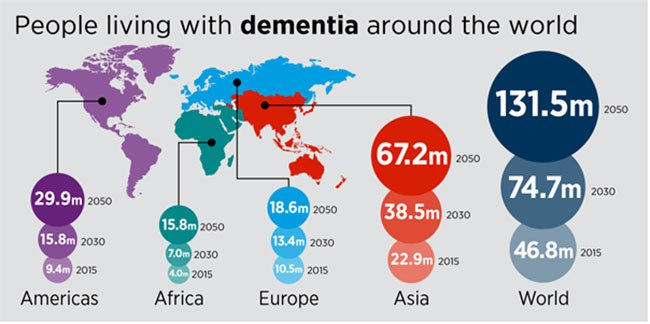
\includegraphics[width=0.7 \textwidth]{images/dementia_globally}
\caption[Prevalence of dementia around the world]{Prevalence of dementia around the world, along with forecasts for 2030 and 2050. Source: \url{http://www.worldalzreport2015.org/}}
\label{fig:adPrevalence}
\end{figure}


\subsection{Symptoms}
\label{sec:bckSym}
% AD, symptoms, age as risk

Symptoms of AD vary depending on the stage of the disease. Some authors \cite{forstl1999clinical} split the symptoms into several categories: pre-dementia stage, mild dementia, moderate dementia and severe dementia. 

\subsubsection{Pre-dementia Phase}

In the pre-dementia stage, the first symptoms are usually attributed to stress and ageing. Careful neuropsychological investigations may reveal very mild cognitive impairment five years before the establishment of clinical diagnosis \cite{forstl1999clinical}. The performance of complex tasks might be reduced, and alterations of behaviour including social withdrawal and depressive dysphoria might also be already present \cite{forstl1999clinical}. 

\subsubsection{Mild Dementia Stage}

In the mild dementia stage, significant impairment of learning and memory are present \cite{forstl1999clinical}. However, short-term and implicit memory are less affected compared to declarative memory. Neuropsychological tests can reveal problems with object naming \cite{chobor1990semantic,locascio1995cognitive}, semantic difficulties with word generation \cite{chobor1990semantic,locascio1995cognitive} and inability to draw figures (i.e. constructional apraxia) \cite{moore1984drawing}. Non-cognitive disturbances are also present at this stage \cite{haupt1992psychopathologische}, where depression has been observed in these mild stages \cite{burns1990psychiatric}.

\subsubsection{Moderate Dementia Stage}

At the moderate dementia stage, the predominant features are severe short-term memory impairment \cite{beatty1988retrograde}, along with difficulties in logical reasoning, planning, language \cite{romero1995pragmatische}, reading \cite{cummings1986pattern} and writing \cite{neils1989descriptive}. More complex actions and activities such as using household appliances, dressing and eating are gradually lost. Vision-related symptoms triggered by cognitive deficits also develop, such as spatial disorientation, inability to recognise familiar faces or illusionary misidentification \cite{reisberg1996behavioral}. Around 20\% of patients also experience visual hallucinations, which may be associated with cholinergic deficits \cite{perry1990visual}.

Patients at this stage cannot survive in their community without help from caregivers. However, hospital or nursing home admission can be delayed if there is a good support system in place at the patient's home. 

\subsubsection{Severe Dementia Stage}

Specific cognitive dysfunctions cannot be disentangled at this stage, due to widespread cognitive deficits. Language is reduced to simple phrases. However, emotional signals can still be received and returned \cite{forstl1999clinical}. Patients need support for performing basic functions such as eating. 

The average life expectancy after clinical diagnosis is between three to nine years, although the speed of progression can vary \cite{querfurth2010mechanisms}. Pneumonia, myocardial infarction and septicaemia are the most frequent causes of death at this stage.

\subsection{Disease Causes and Mechanisms}
\label{sec:bckCau}

The causes for AD are poorly understood and around 70\% of them are thought to be genetic, with many genes involved which include APOE, GSK3$\beta$ and DYRK1A\cite{Ballard2011alzheimers}. Over the last few decades, several hypotheses have been proposed to explain the mechanisms of AD: amyloid hypothesis, tau hypothesis, cholinergic hypothesis and neurovascular hypothesis.


\subsubsection{Amyloid Hypothesis}
\label{sec:bckAmyHyp}

\begin{figure}
\centering
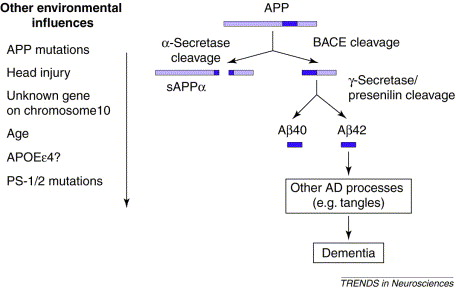
\includegraphics[width=0.6\textwidth]{images/amyloid_hypothesis}
\caption[Diagram showing the amyloid hypothesis]{Diagram showing the amyloid hypothesis. Amyloid precursor protein is split by $\alpha$-secretase resulting in sAPP$\alpha$, which might have a neuroprotective role. On the other hand, splitting by $\beta$-amyloid cleaving enzyme (BACE) results in amyloid-$\beta$, of which amyloid-$\beta$42 is more prone to self-aggregate and lead to pathogenesis. On the left, many other factors are shown that are believed to influence this pathway and lead to more pathology. Reproduced with permission from \cite{mudher2002alzheimer}.}
\label{fig:bckAmyloidHypothesis}
\end{figure}

In 1991, Hardy et al. \cite{hardy1991amyloid} postulated that amyloid-$\beta$ deposits are a central cause in the development of AD. The amyloid-$\beta$ protein, derived from the amyloid precursor protein (APP), is processed via two distinct pathways: the amyloidogenic pathway which produces amyloid-$\beta$ proteins (Fig \ref{fig:bckAmyloidHypothesis}) and the non-amyloidogenic pathway which prevents the formation of amyloid-$\beta$ and instead produces a secreted form of APP called sAPP$\alpha$ \cite{mudher2002alzheimer}. The amyloid hypothesis states that dysregulation in APP processing occurs early in the disease process, causing increased production of the more toxic amyloid-$\beta$42 protein, which aggregates into plaques \cite{mudher2002alzheimer}. The misfolded amyloid-$\beta$ then causes a chain of events leading to cognitive impairment, including tau aggregation, phosphorylation, neuronal damage and brain atrophy. However, the underlying mechanisms through which amyloid-$\beta$ induces neurodegeneration are not clear \cite{mudher2002alzheimer}. 

Different sources of evidence exist to support the amyloid hypothesis. First of all, mutations in the APP gene cause a rare, early-onset form of familial Alzheimer's disease which corresponds clinically and pathologically to AD. This suggests that changes in APP are an upstream \footnote{happening early in the chain of events leading to AD} event in the pathological cascade leading to AD \cite{mudher2002alzheimer}. Moreover, a locus on chromosome 10 which is linked to late onset AD is also associated with increased amyloid-beta production \cite{ertekin2000linkage}. 

Several studies have also established a clear link between amyloid and tau toxicity, another early event in the AD cascade \cite{gotz2001formation, lewis2001enhanced, roberson2007reducing, bloom2014amyloid}. Amyloid has been shown to enhance tau tangle formation in several mice studies \cite{gotz2001formation,lewis2001enhanced}. Evidence also exists that tau pathology is required for amyloid-$beta$ toxicity \cite{roberson2007reducing}, suggesting that there could be a feedback loop between amyloid and tau, or that tau pathology is also required for development of amyloid deficits \cite{bloom2014amyloid}. 

There are several aspects of the amyloid hypothesis that indicate it is not complete. For example, transgenic mouse models carrying the familial AD mutations have showed increases in amyloid toxicity, but no clear evidence of neuronal loss \cite{hsiao1995age,irizarry1997appsw} and tau aggregation as predicted by the amyloid hypothesis \cite{bloom2014amyloid}.

\subsubsection{Tau Hypothesis}
\label{sec:bckTauHyp}

Another key hypothesis about the cause of AD is the tau hypothesis, which  suggests that abnormalities related to the tau proteins initiate the disease cascade \cite{mudher2002alzheimer}. In this case, tau binding to microtubules is disrupted by phosphorylation, which results in free tau that aggregates into neurofibrillary tangles. This ends up destroying the cell's cytoskeleton which collapses the neuron's transport system, ultimately resulting in neuronal death. 

Support for the tau hypothesis was given by the fact that tau proteins aggregate and accumulate within neuronal cells and ultimately cause their death. Moreover, the number of tau tangles has been shown to correlate with cognitive decline \cite{nagy1995relative}, especially in memory-related areas \cite{braak1998evolution,braak1994sequence}. Furthermore, discoveries of tau aggregation in fronto-temporal degeneration (FTD) suggest that tau alone can cause degeneration \cite{heutink2000untangling}.  

There is also evidence that the tau hypothesis is incomplete. For example, the fact that mutations in tau-related genes give rise to tau tangles but no plaques, yet mutations in the APP gene result in both plaques and tangles suggest that amyloid toxicity might occur upstream, before tau toxicity \cite{mudher2002alzheimer}. 

\subsubsection{Cholinergic Hypothesis}
\label{sec:bckChoHyp}

An older hypothesis, on which current AD therapies rely, is the cholinergic hypothesis, which suggests that degeneration of cholinergic neurons and associated disruption of cholinergic neurotransmission are the main causes of pathology in AD \cite{francis1999cholinergic}. Support for the theory came in mid-1970s, where studies provided evidence of deficits in synthesis of neurotransmitter acetylcholine (ACh) and choline acetyltransferase (ChAT) \cite{davies1976selective}. However, the cholinergic hypothesis lost support due to unsatisfactory results of the cholinergic drugs \cite{martorana2010beyond}. Despite not being disease-modifying, cholinergic drugs have been shown to provide symptomatic benefits through improved memory and clinical function \cite{martorana2010beyond}.

\subsubsection{Vascular Hypothesis}
\label{sec:bckVasHyp}

A vascular hypothesis has also been proposed for AD \cite{de2004alzheimer}, suggesting that one of the incipient causes is related to vascular abnormalities, which leads to brain hypoperfusion, neurodegeneration and cognitive impairment. One study even indicates that this is an earlier event than amyloid and tau accumulation \cite{iturria2016early}. Evidence supporting this theory has been given by the close associations between dementia and stroke \cite{kalaria2003vascular,meyer2000risk}, cardiac diseases \cite{breteler2000vascular,aronson1990women,polidori2001heart} and atherosclerosis \cite{hofman1997atherosclerosis}.

\subsubsection{Genetic Causes}
\label{sec:bckGen}

\begin{figure}
\centering
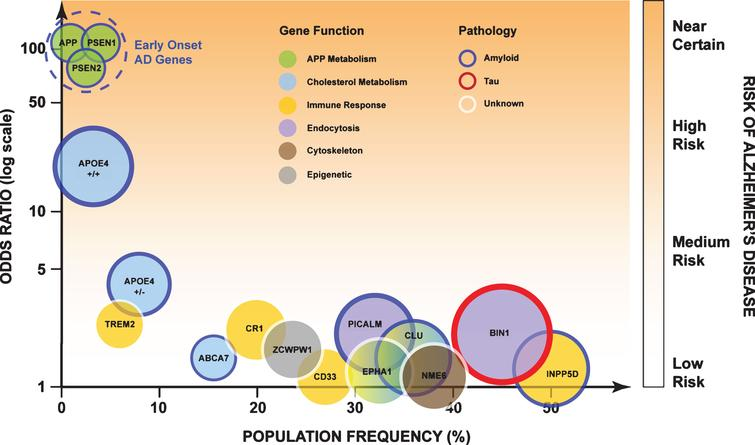
\includegraphics[width=0.9\textwidth]{images/adGenesMap}
\caption[Different genes and associated risk for AD]{Diagram showing different genes which increase the risk for AD (y-axis), as well as their frequency within the population (x-axis). EOAD genes APP, PSEN1 and PSEN2 (top-left) give a near-certain risk of developing AD, but are found in a very small minority of the AD population. APOE4 has a moderate risk, while the other genes have a lower risk, yet are found in a much larger population. Reproduced from \cite{robinson2017recent}, CC BY-NC.}
\label{fig:bckAdGenesMap}
\end{figure}

Alzheimer's disease has a strong genetic component, with many genes involved that alter the risk of developing the disease and the pace of progression. Twin studies show that disease heritability ranges between 60\% to 80\% \cite{bergem1997role,gatz1997heritability}. Currently there are two main forms of AD: familial AD and sporadic AD. Familial AD is a rare early-onset AD (EOAD) characterised by autosomal dominant disease transmission, and caused by mutations in three genes, APP, PSEN1 and PSEN2, which code for amyloid peptide precursor, presenilin 1 and 2 respectively \cite{chouraki2014genetics}. Sporadic AD is the most common, late-onset form of AD (LOAD), characterised by more complex, non-Mendelian transmission. 

In familial AD, several genetic risk factors have been identified so far. In 1980s, the discovery of amyloid-$\beta$ peptides in AD senile plaques and the identification of these peptides in the brains of people with Down's Syndrome, caused by abnormalities in chromosome 21 and where dementia was also observed, led the the hypothesis that mutations of a gene located on chromosome 21 might cause AD in people without Down's syndrome \cite{glenner1984alzheimer}. A few years later, a linkage peak was indeed found on chromosome 21 \cite{st1987genetic}, and the APP gene was identified \cite{goldgaber1987characterization} and confirmed in EOAD families \cite{chartier1991early}. However, the amount of heterogeneity observed in EOAD suggested additional genes were involved, and further genetic linkage analyses led to the discovery of PSEN1 \cite{sherrington1995cloning} and PSEN2 genes \cite{levy1995candidate}. As of March 2014, 40, 197 and 25 mutations were reported in APP, PSEN1 and PSEN2 genes respectively, all with autosomal dominant transmission with complete penetrance, with the exception of one mutation in the APP gene \cite{chouraki2014genetics}.

In sporadic, late-onset AD, the genetic landscape is much more complex. The most important risk factor is given by mutations in genes coding for Alipoprotein E (APOE) \cite{chouraki2014genetics}.  APOE is a protein whose key function is to transport lipids and cholesterols throughout the body, and has three major isoforms called APOE2, APOE3 and APOE4, corresponding to alleles $\epsilon2$, $\epsilon3$ and $\epsilon4$. Increased risk of AD due to APOE4 has been established in 1993 in three key studies \cite{strittmatter1993apolipoprotein, saunders1993association, corder1993gene}. Until 2005, more than 500 candidate genes other than APOE have been identified using association studies, with various pathways involved including tau phosphorylation, vacuolar sorting, glucose and insulin metabolism, nitrous oxide synthesis, oxidative stress, growth factors, inflammation and lipid-related pathways \cite{chouraki2014genetics}.  However, after the advent of genome-wide association studies (GWAS) in 2005, the first genes outside the APOE locus were identified in two independent studies \cite{harold2009genome,lambert2009genome}. Several genes including CLU \cite{harold2009genome,lambert2009genome}, CR1 \cite{lambert2009genome}, BIN1 \cite{seshadri2010genome}, PICALM \cite{harold2009genome}, ABCA7 \cite{hollingworth2011common} and CD2AP \cite{naj2011common} have been since identified. Moreover, associations were also found with quantitative endophenotypes, which provide more statistical power than yes/no disease status, such as early age of onset \cite{thambisetty2013alzheimerA, thambisetty2013alzheimerB}, greater burden of amyloid pathology \cite{biffi2012genetic,chibnik2011cr1}, abnormal levels of cerebro-spinal fluid (CSF) \cite{elias2013genetic, kauwe2011fine}, decrease in total brain volume \cite{bralten2011cr1, furney2011genome} and decreased cognitive scores \cite{barral2012genotype,chibnik2011cr1,mengel2013clu}.


\subsection{Other Risk Factors}
\label{sec:bckRisFac}
% Inflammation,  vascular disease, other risk factors: pollution, smoking

\begin{figure}
\centering
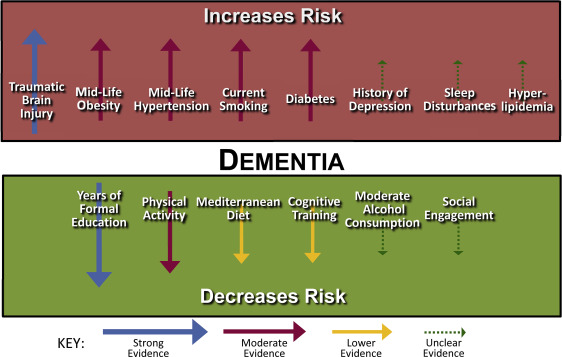
\includegraphics[width=0.6\textwidth]{images/adRiskFactors}
\caption[Different risk factors for AD related to lifestyle and the associated level of evidence]{Diagram showing different risk factors for AD related to lifestyle and the associated level of evidence. Reproduced from \cite{baumgart2015summary}, CC-BY-NC-ND.}
\label{fig:bckAdRiskFactors}
\end{figure}

There are several known risk factors that are associated with AD. The principal risk factor is age, with incidence rates doubling every 5 years after 65 years of age \cite{querfurth2010mechanisms,todd2013survival}. Other risk factors include head injuries, depression and hypertension \cite{Burns2009}. Lifestyle factors such as smoking \cite{cataldo2010cigarette} also increase the risk for developing AD. There is  also potential evidence that living in polluted areas increases the risk for AD \cite{moulton2012air}. Physical exercise is also associated with lower risk of developing dementia \cite{ahlskog2011physical}. Other factors influencing the risk of dementia are shown in Fig. \ref{fig:bckAdRiskFactors}, and include traumatic brain injury, obesity, hypertension, diabetes (increases risk), with protective factors including higher levels of education \cite{baumgart2015summary}.

\subsection{Biomarkers}
\label{sec:bckBio}

The information in this section has been initially written by me for the TADPOLE Challenge website\footnote{\url{https://tadpole.grand-challenge.org/Data/}}, with feedback from Esther E. Bron and Daniel C. Alexander. The material has been subsequently adapted for this thesis. 

Over the last decades, various biomarkers have been developed to quantify the severity of Alzheimer's disease and track its progression:
\begin{itemize}
\item Cognitive tests such as the Mini-Mental State Examination (MMSE) \cite{mckhann1984clinical} are used to assess memory and cognitive performance (section \ref{sec:bckCog}). 
\item Magnetic Resonance Imaging (MRI) measures such as cortical volumes, thickness and atrophy rates detect shrinkage of individual brain areas that is caused by neurodegeneration (section \ref{sec:bckMri}). 
\item Positron Emission Tomography: can be used to measure neuronal metabolism through Fluorodeoxyglucose (FDG) PET \cite{herholz2012use}, amyloid uptake through the Pittsburgh compound B (PiB). \cite{klunk2004imaging} and, more recently, tau uptake through AV1451 PET (section \ref{sec:bckPet}).
\item Cerebro-spinal fluid markers: can be used to measure amyloid plaque deposits \cite{blennow2003csf} and neurofibrillary tangles through CSF total tau and phosphorylated tau \cite{blennow2003csf} (section \ref{sec:bckCsf}).
\end{itemize}

\subsubsection{Cognitive Tests}
\label{sec:bckCog}

\begin{figure}
\centering
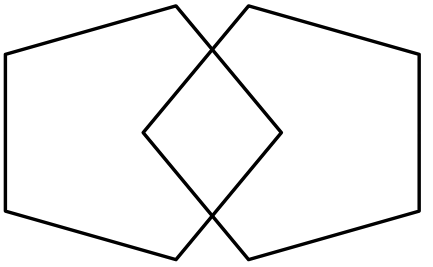
\includegraphics[width=0.3\textwidth]{images/mmse_pentagons}
\caption[Intercalated pentagons used in the Mini-Mental State Examination (MMSE)]{Intercalated pentagons used in the Mini-Mental State Examination (MMSE). Patients with dementia have difficulty drawing them. Image source: Wikipedia\footnotemark \ CC-SA.}
\label{fig:bckMmsePentagons}
\end{figure}
\footnotetext{\url{https://commons.wikimedia.org/wiki/File:InterlockingPentagons.svg}} 

Cognitive tests are neuropsychological tests performed by a clinical expect and can assess different cognitive domains such as general cognition, memory, language, vision. These give an overall sense of whether subjects are aware of their symptoms, surrounding environment and whether they can remember a short list of words, follow instructions and do simple calculations. For instance, in the Mini-Mental State Examination (MMSE), patients are asked to draw intercalated pentagons (Fig \ref{fig:bckMmsePentagons}). As there are no population standards, performance in many of these tests is measured relative to a control group, after adjusting for age, sex and education \cite{mckhann1984clinical}.

Cognitive tests are important in Alzheimer's disease because they measure cognitive decline in a direct and quantifiable manner. As a result, they are required for establishing a clinical diagnosis of probable AD in criteria such as NINCSD-ADRDA \cite{dubois2007research,dubois2010revising}. Apart from establishing the AD diagnosis, these tests are valuable also for establishing patterns of cognitive impairment, assessing changes over time, comparing drug efficacy and for establishing correspondences with other imaging, histopathology or molecular biomarkers \cite{mckhann1984clinical}. 

Cognitive tests have several limitations. First of all, they suffer from practice effects, i.e. patients who undertake the same test several times can learn/remember how to do it, and thus score higher at a follow-up visit. This limits the usefulness of the test in assessing dementia. Another limitations is that they have floor or ceiling effects, which means that many subjects might score the highest/lowest score possible. Finally, they can also be biased, as each subject is evaluated by a human expert who might be influenced by prior knowledge of the subject's cognitive abilities.

\subsubsection{Magnetic Resonance Imaging}
\label{sec:bckMri}

\begin{figure}
\centering
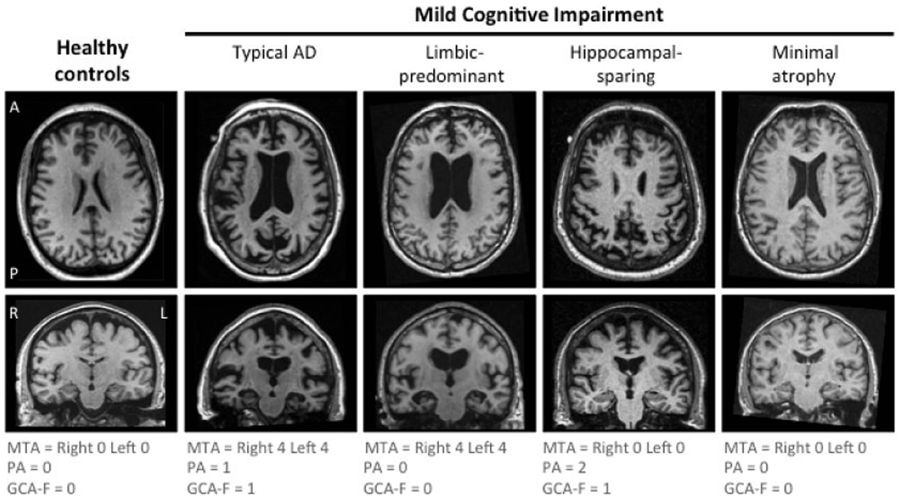
\includegraphics[width=1.0\textwidth]{images/adAtrophy3}
\caption[Comparison between the MRI brain scans of healthy subjects and subjects with mild cognitive impairment]{Comparison between the MRI brain scan of a healthy subject (left) and subjects with different types of mild cognitive impairment (MCI) (middle-right), showing different patterns of atrophy for each group. MRI is a widely used technology for measuring the spatial distribution and extent of atrophy and for tracking the progression of Alzheimer's disease (AD). Reproduced from \cite{ekman2018t}, CC-BY license.}
\label{fig:bckAdAtrophy}
\end{figure}

Magnetic resonance imaging (MRI) is a technique used to image the anatomy and the physiological processes of the brain and other body parts. With MRI, brain structures can be quantified due to different contrast between gray matter (GM), white matter (WM), cerebrospinal fluid (CSF) and hard tissue such as the skull. The GM is the brain tissue that consists of the bodies of neurons, while the WM consists of fibres connecting the neurons. The cerebrospinal fluid is a clear, colourless fluid providing mechanical and immunological protection to the brain. Within MRI, different types of contrast between tissues can be obtained through T1, T2, T1-weighted and T2-weighted images. 

Brain MRI has been successfully applied to quantify neurodegeneration in Alzheimer's disease. Brain atrophy, which is caused by the death of neurons, can be visually assessed in MRI scans due to shrinkage of the brain (see Fig. \ref{fig:bckAdAtrophy}) and can be quantified using markers of volume, cortical thickness, surface areas, along with changes in these values between a baseline and a follow-up scan. These quantitative markers can be obtained with specialised software such as Freesurfer \cite{reuter2012within}.

MRI-derived biomarkers have both advantages and limitations. They are robust and have less noise compared to cognitive tests, and are non-invasive. Moreover, they are also a good indicator of progression from MCI to dementia in an individual subject because they become abnormal slightly earlier than the onset of dementia-specific symptoms \cite{jack2010hypothetical, jack2013update}. Limitations of these markers are that MRI scans are expensive,  require specialised equipment to be acquired, and can also suffer from motion artefacts.

\subsubsection{Positron Emission Tomography}
\label{sec:bckPet}

\begin{figure}
\centering
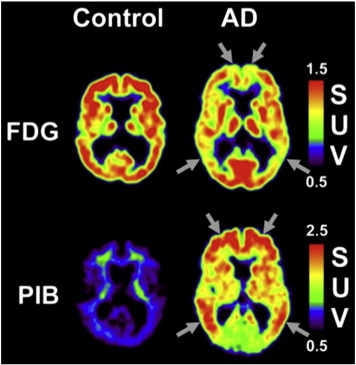
\includegraphics[width=0.4\textwidth]{images/fdgAd}
\caption[FDG PET images of healthy and AD subjects]{(top) Fluorodeoxyglucose (FDG) PET images for a cognitively normal subject (left) and a subject with Alzheimer's disease (right). FDG PET measures cellular metabolism, which is known to decrease during the development of AD. There is decreased metabolism in parietal and frontal regions (gray arrows) in the AD subject compared to the cognitively normal subject. (bottom) Pittsburgh B (PiB) PET image measuring amyloid uptake in the brain of a healthy control (left) and AD subject (right). There is widespread amyloid presence in the brain of the AD subject. Image reproduced with permission from \cite{cohen2014early}.}
\label{fig:bckFdgAd}
\end{figure}

Positron Emission Tomography (PET) detects pairs of gamma rays emitted by a radioactive tracer, which is introduced into the body of a biologically active molecule. Three-dimensional images of tracer concentration within the body are then constructed by computer analysis. Before a PET scan, the patient is injected with a contrast agent (containing the tracer) which spreads throughout the brain and binds to abnormal proteins (amyloid and tau). This enables researchers to track the concentration of these proteins. PET scans can be of several types, depending on the cellular and molecular processes that are being measured:
\begin{itemize}
\item cell metabolism using Fluorodeoxyglucose (FDG) PET: Neuronal cell metabolism refers to the the activity going on inside neuronal cells such as the processing of food and elimination of waste. Metabolic processes use glucose, hence FDG PET quantifies metabolism by measuring the amount of glucose within each voxel. In Alzheimer's disease, neurons that are about to die will show reduced metabolism, hence FDG PET is also an early indicator of neurodegeneration.
\item levels of abnormal proteins such as amyloid-beta through AV45 PET: Amyloid-beta misfolding (i.e. errors in the construction of its 3D structure) is thought to be one of the causes of Alzheimer's disease (see section \ref{sec:bckAmyHyp}). AV45 PET can be used to measure the levels of amyloid in the brain, and is hence one of the earliest AD markers.
\item levels of abnormal tau proteins through AV1451 PET: Abnormal phosphorylated tau (i.e. tau protein and a phosphorus group) that gather together in an insoluble form eventually cause damage to the neuron's cytoskeleton, leading to the collapse of the neuron's transport system and eventually the neuron's death (see section \ref{sec:bckTauHyp}). AV45 PET can be used to measure the level of misfolded tau proteins and is also one of the earliest markers in AD.
\end{itemize}

PET-derived biomarkers are important because they give information about molecular processes that happen in the brain. These are usually the first to become abnormal in the cascade of events that lead to Alzheimer's disease, and are therefore important early markers of the disease that is about to unfold \cite{jack2010hypothetical,jack2013update}.  

PET scans have some limitations that need to be acknowledged. One main limitations is that the patient is exposed to ionising radiation, which limits the number of scans they can take in a specific time interval. PET scans also have a much lower spatial resolution compared to MRI scans. One other caveat with AV1451 PET (tau imaging) is that it is a very new tracer that is still under research, with some studies indicating evidence of some off-target binding in some tau conformations found in non-AD tauopathies \cite{lowe2016autoradiographic,marquie2015validating}. 

\subsubsection{Diffusion Tensor Imaging}
\label{sec:bckDti}

\begin{figure}
\centering
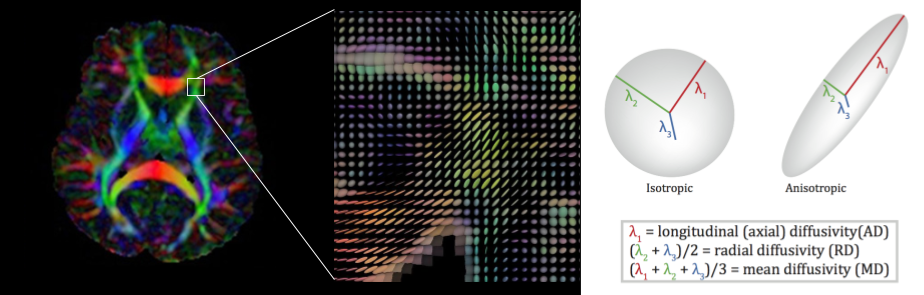
\includegraphics[width=1.0\textwidth]{images/DTI_diagram}
\caption[Diffusion tensor image diagram]{(Left) Diffusion tensor image of a brain showing white matter fibre connections. The colours represent the direction of the connection (red for left-right, blue for superior-inferior, and green for anterior-posterior). (Middle) Zoomed image into the small region of interest (ROI), showing the diffusion tensor ellipses. Each ellipse indicates the direction where water molecules diffused (i.e. moved). (Right) Diagram showing the difference between isotropic diffusion (i.e. equal in all directions) versus anisotropic diffusion, along with the diffusivity measures that can be computed. Diagram assembled by me using images from several sources\footnotemark.}
\label{fig:bckDtiDiagram}
\end{figure}
\footnotetext{
\begin{tabular}{l}
Image sources:\\ 
\url{http://fmri.uib.no/index.php?option=com_content&view=article&id=68&Itemid=86}\\ 
\url{https://commons.wikimedia.org/wiki/File:DTI-axial-ellipsoids.jpg}\\
\url{http://www.diffusion-imaging.com/2012/10/voxel-based-versus-track-based.html}\\
\end{tabular}
}

Diffusion tensor imaging (DTI) is an MRI technique that can be used to measure the degeneration of white matter connections in the brain. This is done by analysing the diffusion of water molecules along the neuron fibre connections. Molecular diffusion in tissues is not free, but reflects interactions with many obstacles, such as macromolecules, fibers, and membranes. When a fiber connection degrades, the diffusion becomes more isotropic (i.e. equal in every direction), which can be quantified using a measure called fractional anisotropy (FA). Fig. \ref{fig:bckDtiDiagram} shows a diagram of a DTI image (left) which is made of diffusion tensors estimated at each voxel (middle). Diffusivities parallel and perpendicular to the fiber direction can then be measured (right).   

DTI is important for analysing the progression of Alzheimer's disease. It has been shown that AD affects white matter bundles \cite{sachdev2013alzheimer}. DTI has also shown great potential for aiding the diagnosis of dementia \cite{bozzali2002white,zhang2009white}. DTI tractography is also important for building brain structural connectomes which have been shown to be disrupted by different types of dementias including Alzheimer's disease \cite{seeley2009neurodegenerative, zhou2012predicting}.

DTI measures have some limitations. As with other MRI modalities, it is susceptible to motion artefacts and suffers from partial volume effects, i.e. measures at each voxel are biased due to averaging across many different cells and types of tissue that are contained in that voxel. Another limitation is that changes in DTI-derived measures such as FA are not specific, and can be attributed to many changes in the underlying cytoarchitecture, such as neurite density or dispersion \cite{zhang2012noddi}. 

\subsubsection{Cerebrospinal Fluid Markers}
\label{sec:bckCsf}

\begin{figure}
\centering
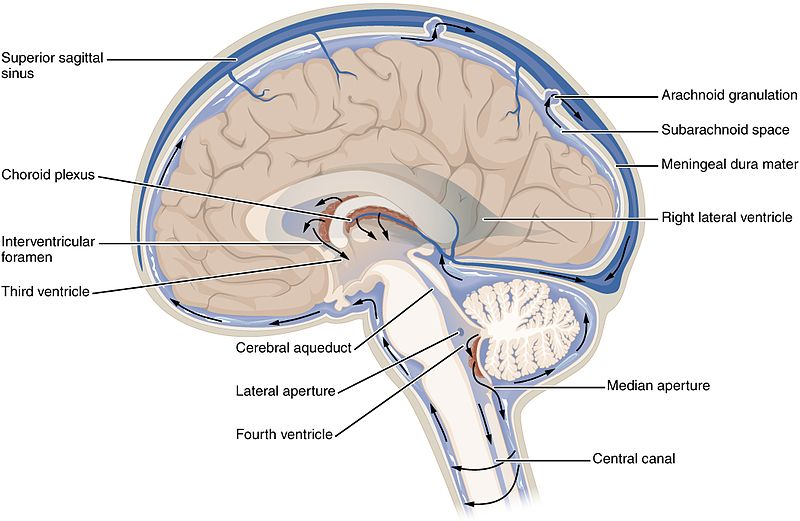
\includegraphics[width=0.5\textwidth]{images/CSF_diagram}
\caption[Diagram showing the cerebro-spinal fluid (CSF).]{Diagram showing the cerebro-spinal fluid (CSF) coloured in blue, which is found in the subarachnoid space around the brain and spinal cord. Source: Wikipedia\footnotemark, CC license.}
\label{fig:bckCsfDiagram}
\end{figure}
\footnotetext{\url{https://en.wikipedia.org/wiki/File:1317_CFS_Circulation.jpg}}

The cerebrospinal fluid (CSF) is a clear, colourless body fluid found in the brain and spinal cord. It acts as a cushion or buffer for the brain, providing basic mechanical and immunological protection to the brain inside the skull. A sample of the CSF can be taken from patients invasively through lumbar puncture, which involves inserting a needle in the spinal cord.

Measures of CSF are very important for dementia research. In the CSF, the concentration of abnormal proteins such as amyloid-beta and tau is a strong indicator of AD. Abnormal levels of concentrations in these proteins are some of the earliest signs of Alzheimer's disease and can indicate abnormalities many years before symptom onset \cite{jack2010hypothetical}.

The CSF measures have some limitations. One key limitation is that the lumbar puncture is highly invasive and thus not performed in many studies. The CSF measures are also not specific to any particular part of the brain.

\subsection{Diagnosis}
\label{sec:bckDia}

A diagnosis of Alzheimer's disease is usually given based on the person's medical history, behaviour and information provided by the relatives. Medical imaging from Magnetic Resonance Imaging (MRI), Computer Tomography (CT) or Positron Emission Tomography (PET) can help exclude other types of brain pathologies or types of dementia. Memory tests from neuropsychological batteries can help characterise the stage of the disease \cite{waldemar2007recommendations}.

The most commonly used diagnostic criteria are from the National Institute of Neurological and Communicative Disorders and Stroke (NINCDS) and the Alzheimer's Disease and Related Disorders Association (ADRDA) \cite{dubois2007research,dubois2010revising}. This criteria, commonly called NINCSD-ADRDA, require evidence of cognitive impairment through neuropsychological testing for establishing a clinical diagnosis of \emph{probable} AD, while histopathologic confirmation is required for definite confirmation \cite{dubois2007research,dubois2010revising}.


\section{Progression of Alzheimer's Disease}
\label{sec:bckProgAd}

% disease progression in AD
Several studies have been done so far on Alzheimer's disease progression \cite{jack2010hypothetical, ridha2006tracking,fox1999correlation, scahill2002mapping, braak1991neuropathological,schott2003assessing}. It is currently believed that abnormal changes in amyloid-beta and tau aggregation happen very early, long before symptoms occur, followed by hypometabolism and structural atrophy, and then cognitive decline such as memory loss and executive dysfunction \cite{jack2010hypothetical,jack2013tracking}.  Neuropathological staging of AD brains showed that the earliest change in brain structure are in the medial temporal lobe, particularly in the entorhinal cortex and hippocampus \cite{braak1991neuropathological}. This has also been confirmed with in-vivo MRI studies, which showed that even in mild AD the entorhinal area and hippocampus shrink by 20-25\% compared to controls \cite{jack1997medial, lehericy1994amygdalohippocampal, juottonen1999comparative, bobinski1999histological}. Results by Schott et al. \cite{schott2003assessing} and Ridha et al. \cite{ridha2006tracking} show that atrophy of the medial temporal lobe precedes the clinical onset of AD by approximately 3.5 years \cite{schott2003assessing}. 

\subsection{Braak Staging}
\label{sec:bckBraak}

In 1991, Braak and Braak \cite{braak1991neuropathological} proposed a staging system based on the spatial spread of amyloid plaques, neurofibrillary tangles (NFT) and neutropil threads (NT). It was the first attempt to build a staging scale for Alzheimer's disease from neuropathology, using a cross-sectional set of brains and without using clinical information.

The amyloid patterns of the Braak staging system proved to be of limited significance for the differentiation of neuropathological stages \cite{braak1991neuropathological}, but still enabled separation into three stages. In the initial stage, amyloid deposits are found in the basal portions of the isocortex, followed by fast spreading in virtually all isocortical association areas by the middle stage. In the late stage, amyloid plaques are found in all areas of the isocortex, including sensory and motor fields \cite{braak1991neuropathological}.

The spreading of neurofibrillary tangles allowed separation into six key stages. Stages I-II were characterised by mild or moderate accumulation in the transentorhinal layer Pre-$\alpha$\footnote{Pre-$\alpha$ is one of the layers from the principal stratum (Pre) of the entorhinal cortex. It is characterised by cellular islands of large projection cells, and it's connections project to the hippocampus.} \cite{braak1991neuropathological}. Afterwards, stages III-IV were marked by the spread of NFTs into the transentorhinal region and proper entorhinal cortex, along with mild involvement of the first Ammon's horn sector \cite{braak1991neuropathological}. Finally, stages V-VI were marked by the spread of NFTs and NTs to almost all isocortical association areas. \cite{braak1991neuropathological}

\subsection{Neuroimaging}
\label{sec:bckNeu}

In AD, Magnetic Resonance Imaging (MRI) shows gray matter atrophy throughout the brain, in particular in the hippocampus and entorhinal cortex \cite{whitwell2010progression}. In terms of atrophy progression, it starts in the medial temporal lobe and fusifom gyrus at least 3 years before an AD diagnosis, and then spreads to the posterior temporal lobe, parietal lobe, and finally to the frontal lobe. However, the sensorimotor cortex, visual cortex and the cerebellum are relatively spared \cite{whitwell2010progression}.  

Imaging with Positron Emission Tomography (PET) shows reduced metabolism (FDG) and increased uptake of amyloid (e.g. AV45) proteins \cite{marcus2014brain}. In early stages of AD, hypometabolism affects the parietotemporal association areas, the posterior cingulate gyrus and the precuneus. In later stages, frontal cortices also become affected, while the striatum, thalamus, primary sensorymotor cortices, visual cortices and the cerebellum seem to be spared \cite{marcus2014brain}. In terms of amyloid deposition through amyloid PET, early deposits are found in the precuneus, orbitofrontal, inferior temporal and posterior cingulate, later followed by the entire prefrontal cortex, lateral temporal and parietal lobes \cite{marcus2014brain}. These patterns have been validated using autopsy studies\cite{clark2011use, clark2012cerebral}. 

\section{Posterior Cortical Atrophy}
\label{sec:bckPca}

\begin{figure}
\centering
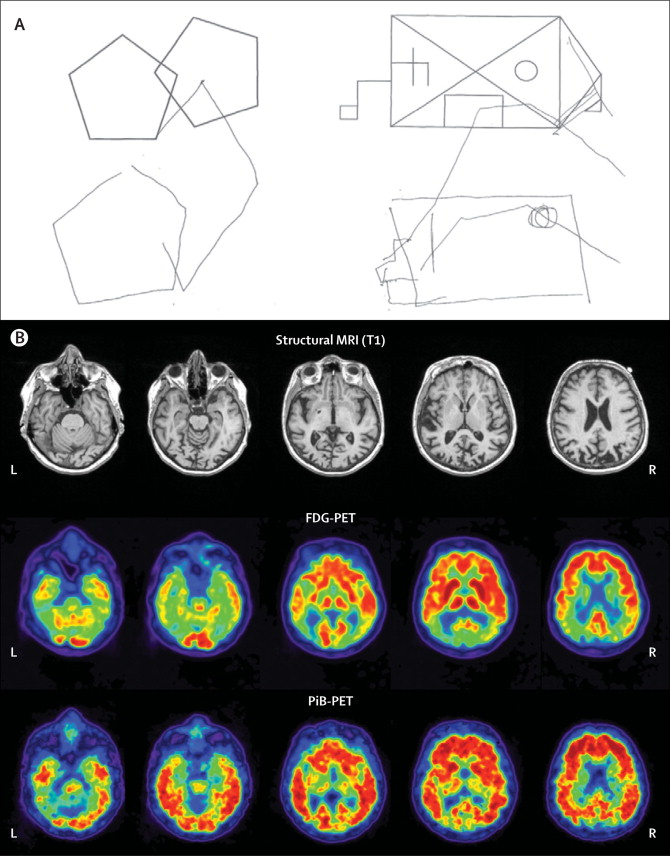
\includegraphics[width=0.8\textwidth]{images/pcaImagingDrawing}
\caption[Visual deficits and neuroimaging pathology in Posterior Cortical Atrophy]{(A) Visual deficits as shown when a 62-year old PCA patient was asked to copy the intersecting pentagons figure \cite{crutch2012posterior}. (B) Structural MRI, FDG PET and PiB PET scans of the same subject. Structural MRI shows atrophy predominant in the bilateral parietal, posterior temporal and lateral occipital regions (B, top), FDG PET shows reduced metabolism in the same regions (B, middle), while PiB-PET shows diffuse amyloid uptake throughout the entire brain (B, bottom) \cite{crutch2012posterior}.  }
\label{fig:bckPcaImg}
\end{figure}

Posterior cortical atrophy (PCA) is an early-onset neurodegenerative syndrome that affects the posterior part of the brain, resulting in the disruption of the visual cortex. The syndrome, also called Benson's syndrome, was first reported by Benson et al. \cite{benson1988posterior} in 1988 to describe five patients with fairly homogeneous but otherwise unclassified symptoms.  

\subsection{Symptoms}
\label{sec:bckPcaSym}

The most common symptoms include general visuospatial and visuoperceptual impairments such as inability to read, blurred vision, light sensitivity, trouble navigating through space and issues with depth perception \cite{crutch2012posterior,borruat2013posterior}. Additional symptoms also include apraxia (disorder of movement planning), visual agnosia (object recognition deficit) and agraphia (loss of writing ability) \cite{benson1988posterior, goethals2001posterior}. These symptoms get worse as the disease progresses, with patients becoming unable to recognise familiar people, objects, difficulty navigating familiar places and drawing (see Fig. \ref{fig:bckPcaImg}). Some studies  \cite{andrade2010visual, andrade2012visuospatial, andrade2013visuospatial} reported visual hemineglect (difficulty seeing one half of the visual field) to be frequent in PCA patients, especially if asymmetrical atrophy takes place in the occipital areas. 

PCA patients report higher-order visual problems related to object and space perception, compared to more basic visual impairments e.g. in colour and motion, although impairments in higher order visual functions might be due to lower-level disruption. One study \cite{lehmann2011basic} reported that all PCA subjects showed impairment in at least one low-level visual process, and that this correlates with higher-order visuospatial and visuoperceptual functions, but not with non-visual functions of the parietal lobe, including calculations and spelling.

\subsection{Causes}
\label{sec:bckPcaCau}

The causes of PCA are still unknown, due to the rarity of the disease, gradual onset of symptoms and no fully accepted diagnostic criteria \cite{borruat2013posterior,crutch2012posterior}. The progressive neurodegeneration that characterises PCA is often attributed to Alzheimer's disease pathology (i.e. aggregation of amyloid plaques and tau tangles), but alternative causes including dementia with Lewy bodies, corticobasal degeneration and prion disease have also been identified \cite{crutch2012posterior}. One study reported the PCA syndrome in a 4-sibling family with prion disease \cite{depaz2012long}, suggesting that prion propagation mechanisms might be involved in PCA.

Genetic factors that underlie PCA are also not well understood \cite{crutch2012posterior,borruat2013posterior}. Empirical findings suggest that there are no significant differences in the number of patients with a positive family history of PCA and typical AD \cite{crutch2012posterior}. Some studies also report no differences in Alipoprotein E (APOE) genotypes between PCA and typical AD \cite{mendez2002posterior, tang2004clinical, rosenbloom2011distinct, migliaccio2009clinical}, although other studies reported differences in APOE $\epsilon$4 allele status, with fewer PCA patients being $\epsilon$4-positive \cite{schott2006apolipoprotein,snowden2007cognitive}. These differences have been attributed to differences in inclusion criteria of PCA with respect to typical AD \cite{crutch2012posterior}.

\subsection{Diagnosis}
\label{sec:bckPcaDia}

PCA patients face difficulties in diagnosis due to the young age at onset and the fact that there are no fully accepted diagnostic criteria. Patients are sometimes misdiagnosed with depression, anxiety or even malingering in early stages of the disease \cite{crutch2012posterior}. They are often initially referred to opticians and ophthalmologists in the belief that ocular abnormalities are causing their visual deficits, often leading to unnecessary medical procedures such as cataract surgery. Neuroimaging modalities such as magnetic resonance imaging (MRI), positron emission tomography (PET) or single photon emission computed tomography (SPECT) can aid diagnosis of PCA \cite{goldstein2011posterior}. 

There are no widely accepted diagnostic criteria, although two criteria have been proposed so far by Mendez et al. \cite{mendez2002posterior} and Tang-Wai et al. \cite{tang2004clinical}. These criteria suggested presence of visual deficits in absence of other eye diseases, gradual progression, relative preservation of anterograde memory, absence of stroke or tumour, and other neuropsychological or imaging abnormalities that are related to parietal or occipital functions. 

However, these criteria have some limitations. They are yet to be thoroughly validated outside their centres, and need to be linked to underlying pathology, otherwise inconsistencies between studies and centres will occur. Moreover, the current criteria provide no guidance to the level of specificity required for a diagnosis of PCA \cite{crutch2012posterior}. It has been suggested that PCA, when caused by underlying AD pathology, lies on a continuum of phenotypical variation between AD and purely-visual PCA, with no clearly defined diagnosis boundary \cite{snowden2007cognitive, migliaccio2009clinical, lehmann2011basic}.

\subsection{Management}
\label{sec:bckPcaMan}

There is no known efficient treatment of PCA that will reverse or stop neurodegeneration \cite{borruat2013posterior}. Patients with PCA are usually treated with the same medication as for AD, namely cholinesterase inhibitors: tacrine, rivastigmine, galantamine and donepezil \cite{borruat2013posterior}. Crutch et al. \cite{crutch2012posterior} suggest that antidepressant drugs might also be appropriate in patients with low mood, and levodopa or carbidopa could aid individuals with Parkinsonism. However, there are no studies analysing the efficiency of these drugs in PCA patients \cite{borruat2013posterior}. 

A few non-pharmacological therapies have also been attempted recently in some patients that included psycho-educative programs \cite{videaud2012impact} or a combination of speech therapy, occupational therapy and physiotherapy \cite{weill2012physical}.

\subsection{Neuroimaging}
\label{sec:bckPcaNeu}

Several MRI studies in PCA have shown damage to posterior brain regions. Studies by Hof et al. \cite{hof1997atypical} and Tang-Wei et al. \cite{tang2004clinical} show a greater concentration of senile plaques and neurofibrillary tangles in the occipital and parietal lobes and at the occipito-temporal junction. Cross-sectional studies using voxel-based morphometry have also shown significant abnormalities in occipital and parietal lobes, followed by the temporal lobe \cite{lehmann2011basic,whitwell2007imaging}. When compared directly to typical AD subjects, PCA have shown greater atrophy in the right parietal lobe and less in the left temporal and hippocampal regions \cite{lehmann2011cortical,crutch2012posterior}. Some DTI studies also seem to suggest white matter damage in posterior regions \cite{duning2009pattern,yoshida2004white,migliaccio2012brain}. See Fig. \ref{fig:bckPcaImg} for MRI scans of a PCA patient, showing the typical posterior pattern of atrophy.

Non-MRI imaging studies in PCA have also shown similarly posterior abnormality patterns. Functional imaging studies using single photon emission computer tomography (SPECT) and FDG PET also show reduced function in occipital and parietal regions \cite{kas2011neural, gardini2011visuo, aharon1999posterior, pietrini1996preferential}. Amyloid pathology, as measured with PiB-PET, has been found in occipital and parietal areas, as compared to typical AD subjects \cite{ng2007evaluating, kambe2010posterior, tenovuo2008posterior, formaglio2011vivo}, although this finding was not confirmed in two other studies, which found more diffuse amyloid uptake \cite{rosenbloom2011distinct,de2011similar}.

\subsection{Heterogeneity}
\label{sec:bckPcaHet}
%TODO: dorsal, ventral, caudal

Some studies \cite{ross1996progressive, galton2000atypical} have shown that there is considerable heterogeneity within PCA itself, where three main PCA subgroups have been reported: primary visual (the striate cortex, caudal), parietal (dorsal) and occipitotemporal (ventral) \cite{ross1996progressive, galton2000atypical}. 

Patients with primary visual subtype showed poor vision deficits, with later problems with memory, attention and presence of visual hallucinations \cite{galton2000atypical,levine1993visual}. Imaging showed reduction in occipital lobe perfusion. In one of the studies, AD diagnosis was confirmed post-mortem, upon pathological examination \cite{galton2000atypical}. However, evidence for the existence of this subgroup is very limited, with only two patients identified so far in different case studies \cite{levine1993visual,galton2000atypical}, with another study having reported no "pure" visual deficits within a cohort of n=21 PCA subjects\cite{lehmann2011basic}.

Patients with the parietal (dorsal) PCA subtype generally show initial visuospatial symptoms, agraphia (inability to draw) and dyspraxia, but have preserved visual fields, basic perceptual abilities, object recognition and reading and show biparietal and occipital deficits, disrupting the dorsal or "where" stream \cite{ross1996progressive,galton2000atypical}. 

Patients with the occipitotemporal (ventral) PCA subtype generally show symptoms related to visual distortion, inability to recognise objects, general topography and written words and show occipitotemporal pathology, disrupting the ventral or "what" stream \cite{ross1996progressive,galton2000atypical}.

While all this evidence suggests that there is considerable heterogeneity within the PCA syndrome, evidence is very limited to a few case studies, with some patients also having no pathological confirmation of underlying AD pathology. Moreover, some \cite{crutch2012posterior,lehmann2011basic} have suggested that these subtypes should not be interpreted as distinct groups, but rather as points on a continuum of phenotypical variation.

\chapter{Background -- Disease Progression Models}
\label{chapter:bckDpm}

\begin{figure}
\centering
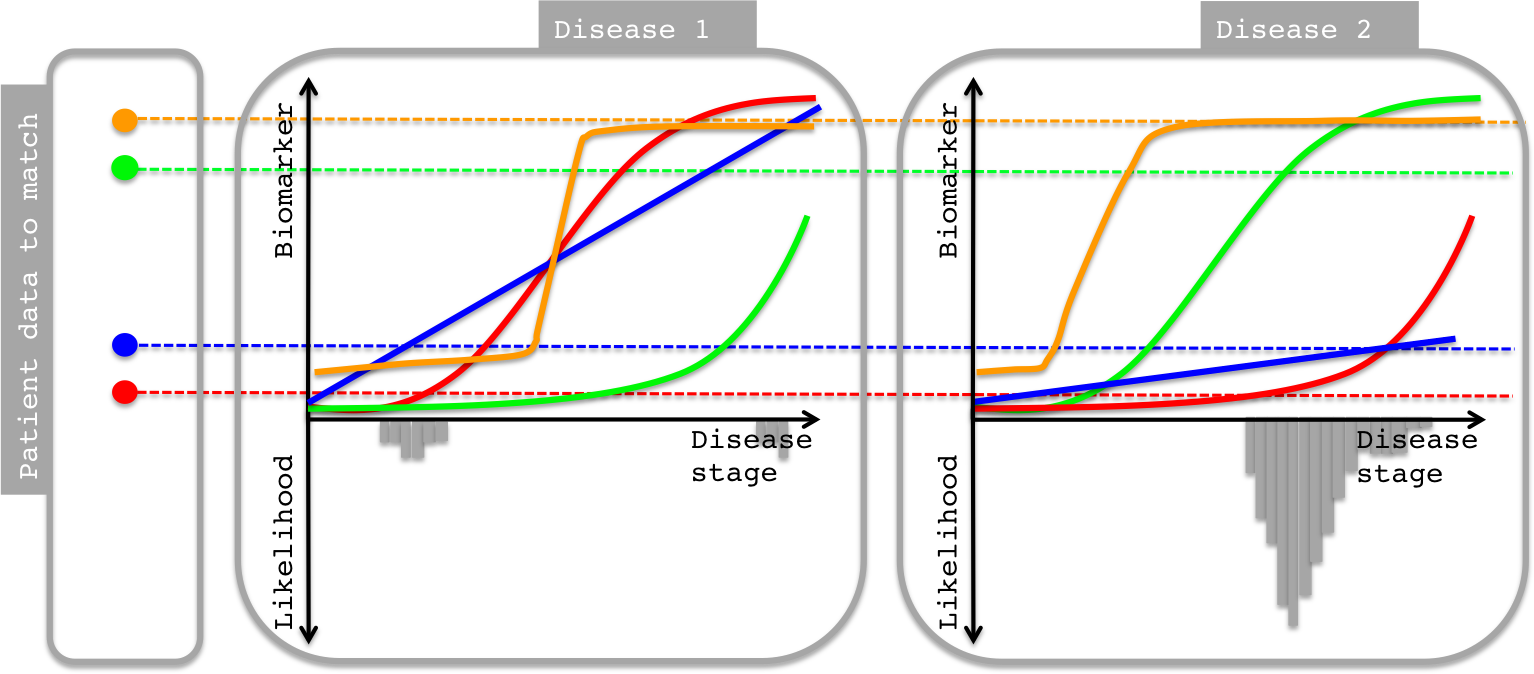
\includegraphics[width=1\textwidth]{images/dpmDiffDiag2}
\caption[Hypothetical biomarker signatures in two diseases]{Cartoon showing hypothetical biomarker signatures from two diseases, along with a cross-sectional snapshot of data from a patient (left). For one patient, disease staging implies finding the optimal time-shift along the horizontal axis that would match its data. On the negative y-axis, the histogram of possible stages is shown. Differential diagnosis can performed by evaluating the integral of the distribution of stages on the negative y-axis, and selecting the disease that has the largest integral. Deriving quantitative biomarker signatures using disease progression modelling can help with disease understanding, staging and differential diagnosis. Image courtesy of Neil Oxtoby and Daniel Alexander.}
\label{fig:bckDpmImg}
\end{figure}

% what is a disease progression model?
A disease progression model is a mathematical model that describes the evolution of biomarkers in a neurodegenerative disease. Such quantitative models promise to enable early and precise diagnosis of dementia before symptoms appear, and will enable stratification of subjects in AD clinical trials. This is important, because it is currently believed that one of the reason why AD clinical trials failed is because treatments were not administered early enough, and to the right patients \cite{mehta2017trials}. Moreover, the advent of large multimodal biomarker datasets containing neuropsychological, imaging, genetic and molecular data can enable the development of specialised progression models that accurately predict the evolution of subjects. 

Quantitative biomarker signatures estimated through disease progression models have several other key benefits, which are illustrated in Fig. \ref{fig:bckDpmImg}. First of all, they enable disease understanding as well as testing and validation of hypotheses regarding underlying disease mechanisms. Secondly, they enable staging of patients along the progression axis (x-axis), along with prognosis estimates, which can be useful in clinical settings. Third, they also enable differential diagnosis by comparing the fit of the patient's data to signatures of different diseases. 

In this chapter we review the disease progression models that have been developed in the literature. We present the hypothetical model by Jack et al. \cite{jack2010hypothetical} (section \ref{sec:bckDpmHyp}), followed by early models of progression based on symptomatic groups (section \ref{sec:bckDpmSym}) and regression against a clinical marker (section \ref{sec:bckDpmReg}). We then review data-driven models of disease progression such as the event-based model \ref{sec:bckEbm}, the differential equation model (section \ref{sec:bckDem}), the disease progression score (section \ref{sec:bckDps}), self-modelling regression (section \ref{sec:bckSem}), the manifold-based model (section \ref{sec:bckMan}), the voxelwise mixed effects model (section \ref{sec:bckVox}) and the network diffusion model (section \ref{sec:bckNet}), as well as discriminative models used normally in machine learning (section \ref{sec:bckMac}).

\section{Hypothetical Models}
\label{sec:bckDpmHyp}

\begin{figure}
 \centering
 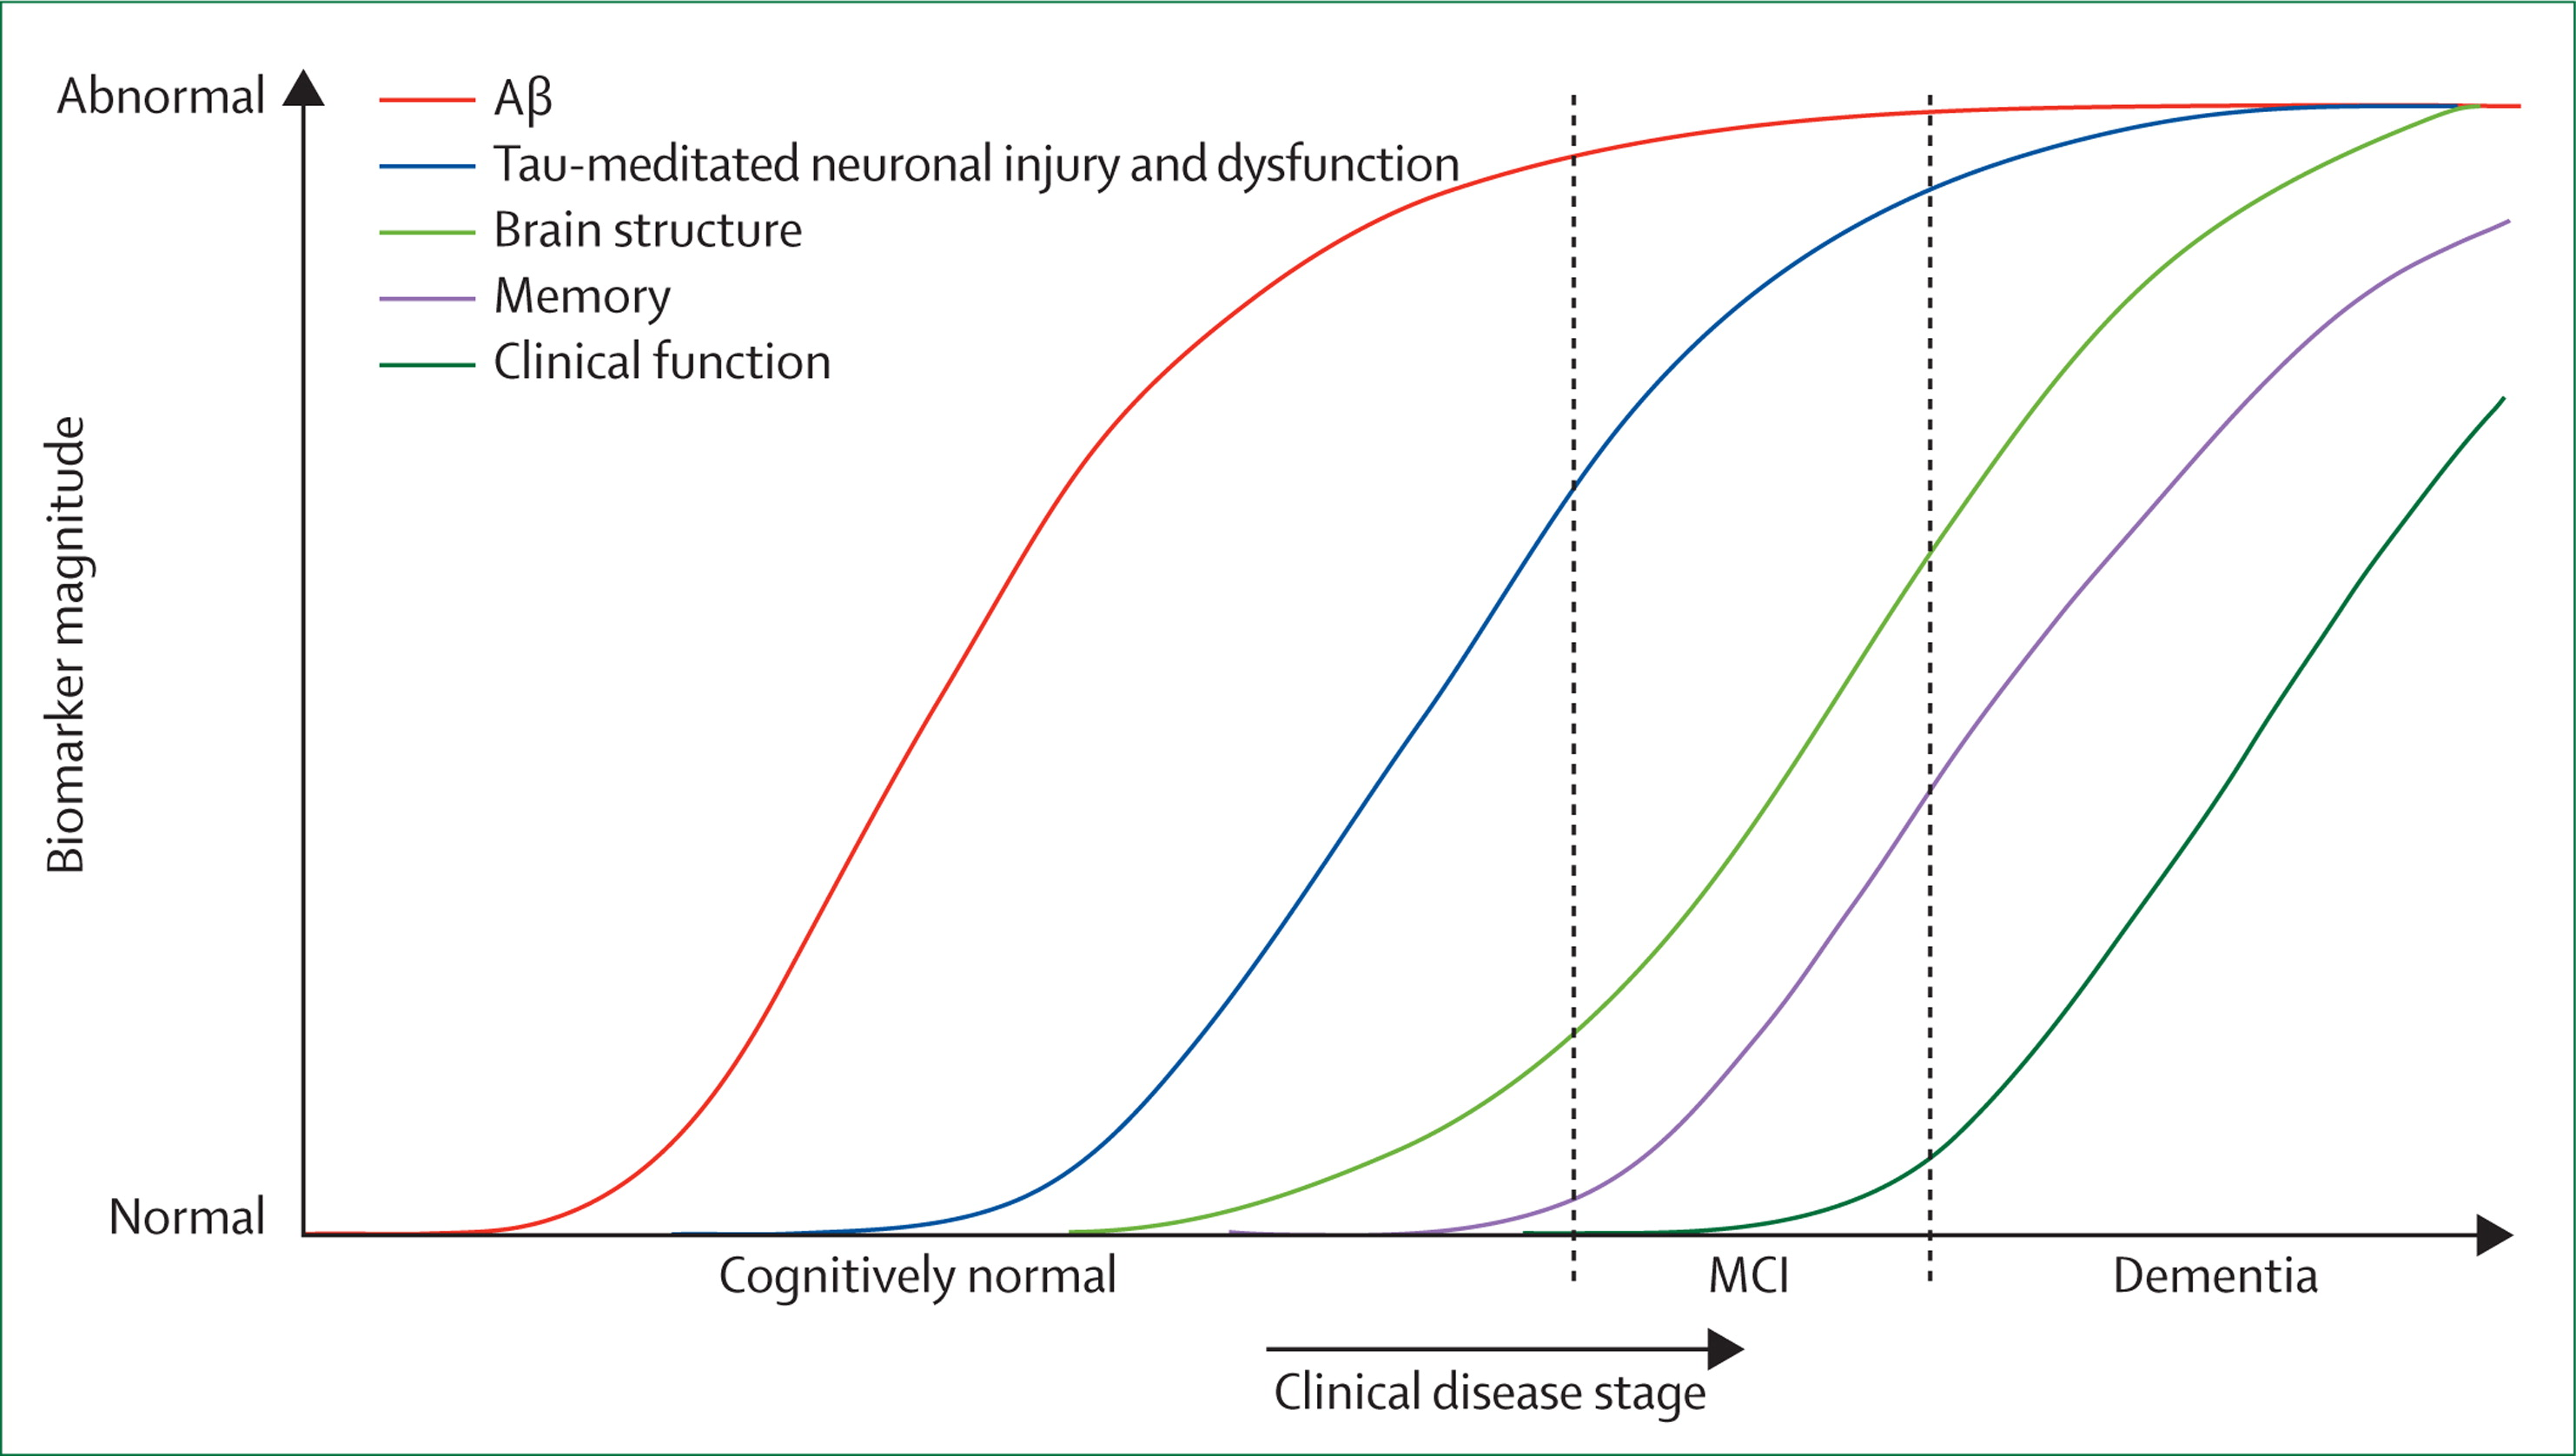
\includegraphics[scale=0.85,trim=5 5 5 5,clip]{images/jackCurves}
 \caption[Biomarker cascade by Jack et al. \cite{jack2010hypothetical}]{Dynamic biomarkers of the AD cascade as hypothesised by Jack et al. \cite{jack2010hypothetical}. A$\beta$ and tau are thought to become abnormal before the onset of any dementia symptoms, while brain structure, memory and clinical function are thought to become abnormal later, during MCI and dementia stages. Reproduced with permission from \cite{jack2010hypothetical}.}
 \label{fig:biomk_cascade}
\end{figure}

% Hypothetical model of disease progression by Jack
A hypothetical model of disease progression has been proposed by Jack et al. \cite{jack2010hypothetical,jack2013tracking}, which describes the trajectory of several key biomarkers during the progression of Alzheimer's disease (fig. \ref{fig:biomk_cascade}). Using aggregated evidence from past literature, the model suggests that amyloid-$\beta$ and tau protein biomarkers become abnormal long before the onset of any dementia symptoms. Afterwards, during the mild cognitive impairment (MCI) phase, cognitive functions such as memory become abnormal along with brain structure measured using MRI. These biomarkers continue to be affected in the dementia stage, while A$\beta$ and tau seem to reach a plateau at this point. This hypothesised model of disease progression is shaping the current field of AD research \cite{donohue2014estimating}.

Apart from placing the biomarkers on a single time frame and suggesting the order in which they become abnormal, the model also made some key observations. First of all, the sequence of abnormality was not assumed to change then stop, rather some biomarkers gradually became abnormal simultaneously, although at different speeds and in an ordered manner. Secondly, amyloid plaques are necessary but not sufficient to develop AD pathology \cite{jack2013update}, with cognitive decline correlating less with amyloid deposition \cite{jack200811c} compared to tau and neurodegenerative markers \cite{hyman2011amyloid}. Third, the authors suggested biomarker trajectories follow non-linear curves, hypothesised to be similar in shape to sigmoids \cite{jack2013update, ridha2006tracking, jack2008atrophy}. Fourth, a time-lag exists between evidence of amyloid pathology and the appearance of cognitive deficits, probably mediated by brain resilience and cognitive reserve \cite{jack2013update}.

The hypothetical model nevertheless has some limitations. First of all, it is a hypothetical, theoretical model that is meant to be a guide for future researchers modelling disease progression in Alzheimer's disease. Hence, the model is not quantitative and cannot be used to e.g. stage patients. Another limitation is that the x-axis (disease progression) and y-axis (biomarker abnormality) are not well-defined. Various implementations that will be discussed next have made various assumptions about how to define this, such as computing Z-scores with respect to controls \cite{jedynak2012computational}, or used percentiles over the observed biomarker values \cite{donohue2014estimating}. In the next sections, we will present the development of quantitative models that address these limitations.

\section{Models of Progression using Symptomatic Groups}
\label{sec:bckDpmSym}

% simple models that regress group patients in clinical symptomatic stages or regress against one variable (years from onset)
Some of the simplest disease progression model are based on symptomatic staging of patients into a small number of groups, e.g. "pre-symptomatic", "mild", "moderate" and "severe" \cite{fonteijn2012event}. They then describe the differences in biomarker measurements among these groups. Scahill et al. \cite{scahill2002mapping} devised such a method that finds changes in brain structure using voxel-based analysis of serial nonlinear-registered MRI images. Other models based on symptomatic staging are those of Dickerson et al., 2009 \cite{dickerson2009cortical} and Thomson et al., 2001 \cite{thompson2001cortical} and 2003 \cite{thompson2003dynamics}. 

These models have several key limitations. First of all, they rely on clinical assessment, which is usually subjective and biased. Secondly, they offer very limited temporal resolution and cannot model changes in pre-symptomatic phases of the disease.   

\section{Regression Against One Biomarker}
\label{sec:bckDpmReg}

In order to estimate longitudinal biomarker trajectories, some authors have proposed regressing against a clinical or age-related marker.  Sabuncu et al. \cite{sabuncu2011dynamics} regressed the cortical thinning rate against MMSE scores. Jack et al. \cite{jack2012shapes} also used regression against MMSE to estimate the shape of biomarker trajectories. Doody et al. \cite{doody2010predicting} regressed biomarkers against time since baseline visit. Driscoll et al. \cite{driscoll2009longitudinal} estimated brain volume trajectories using a mixed effects model against age, using other demographic variables such as gender and intracranial volume (ICV) as covariates. 

These methods have some limitations. Regression methods against clinical markers are limited by the fact that they cannot estimate biomarker dynamics in pre-clinical stages. On the other hand, regression against age or time since baseline visit assume that all subjects have the same age of disease onset or that disease onset is at baseline visit.

Another method for estimating biomarker trajectories, which is popular in familial AD, performs non-linear regression of mutation carriers' data against estimated years from parent's onset \cite{bateman2012clinical, benzinger2013regional}. However, this method can only be applied to dominantly inherited AD, which represents only a small percentage of the entire AD population.

\section{Survival Analysis Models}
\label{sec:bckDpmSur}

Survival analysis models are a class of models used to predict time until an event, in this case conversion to mild cognitive impairment (MCI) or AD. One popular type of survival model in AD is the Cox proportional hazards model, which assumes a multiplicative increase in the hazard rate with respect to a unit-increase in the covariate. Cox proportional hazards models have been used to estimate the probability of progression to AD in a variety of studies \cite{young2014data, dickerson2011alzheimer, bouwman2007csf, csernansky2005preclinical, hansson2006association, kawas2003visual}. A related model is the proportional odds model, which is more suitable for discrete data, and has also been applied to evaluate risk of developing in AD \cite{stoub2005mri, jack200811c, vemuri2009mri}.

Non-parametric survival models such as the Kaplan-Meyer estimator have also been used \cite{morris2001mild, modrego2004depression, carr2000value, khachaturian2004apolipoprotein}. However, the Kaplan-Meyer method can only use a single, binary predictor variable as opposed to the Cox regression method.

The main limitation of survival models is that they require accurate and reliable diagnostic classes, which are not always available and can sometimes be inaccurate due to human errors.


\section{Scalar Biomarker Models}
\label{sec:bckSca}

% Disease progression - EBM
Over the last few years, a range of latent-time models of disease progression have also been proposed, which estimate scalar biomarker trajectories without relying on a-priori defined cognitive groups, diagnosis or clinical markers. Here, by latent-time models we mean models that estimate a latent temporal dimension of disease progression in an unsupervised manner. In this section we will present several such models: the event-based model (section \ref{sec:bckEbm}), the differential equation model (section \ref{sec:bckDem}), the disease progression score model (section \ref{sec:bckDps}), the self-modelling regression model (section \ref{sec:bckSem}) and the manifold-based mixed effects model (section \ref{sec:bckMan}). These models use scalar biomarker values which are assumed to be uncorrelated, as opposed to more complex spatial data such as brain images or cortical shapes.

The main premise behind there models is that they assume measurements are taken from subjects who are at various unknown points along the progression of the same disease. The models attempt to estimate simultaneously differences in the dynamics of the disease progression while also estimating the time shift and progression speed along the disease timeline, also called temporal heterogeneity. Some models go a step further and also estimate differences that are due to spatial heterogeneity of the subjects, using random effects estimating deviations from the population trajectory. Such combined modelling is challenging, as it introduces identifiability issues. 


\subsection{The Event-Based Model}
\label{sec:bckEbm}

\begin{figure}
\begin{tikzpicture}[scale=1.4, every node/.style={scale=1}]

\node (tab1) at (-3,2.5) {
\begin{tabular}{c | c | c | c}
& Patient 1 & Patient 2 & Patient 3\\
\hline
  Region 1 & 1.1 & 0.9 & 0.1\\
  Region 2 & 0.95 & 0.0 & 0.05\\ 
\end{tabular}
};
\node (fig1) at (-2.5,0) {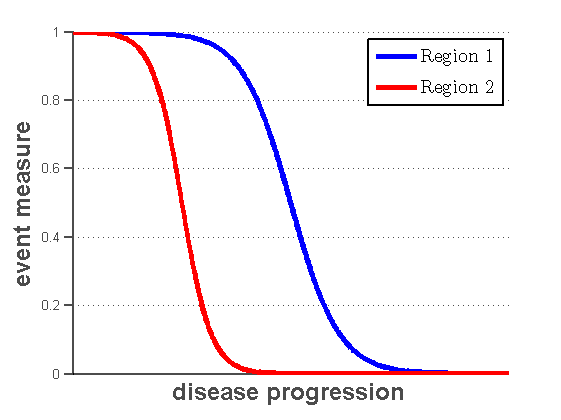
\includegraphics[height=5.0cm]{images/ebmMethod2Biomk}}; 
\draw[-,line width=0.4mm,] (-3.75,2) -- (-3.75,-1.5);
\draw[-,line width=0.4mm,] (-2.4,2) -- (-2.8,1.5) -- (-2.8,-1.5);
\draw[-,line width=0.4mm,] (-1.1,2) -- (-1.9,1.5) -- (-1.9,-1.5);


\node (mixModel) at (1.8,2.5) {
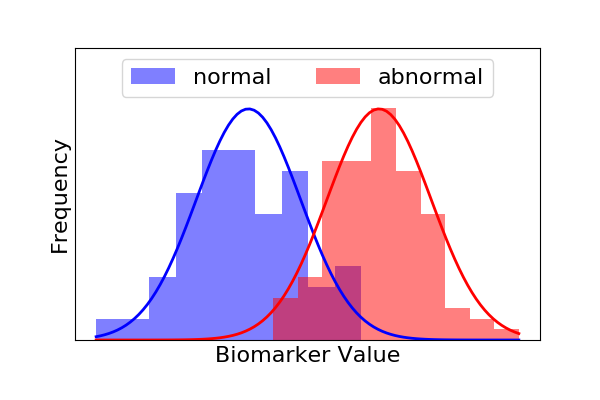
\includegraphics[height=3cm]{images/abnormal1.png}};
\node (mixModelLabel) at (mixModel.north) {Region 1};
\node (mixModel2) at (4.6,2.5) {
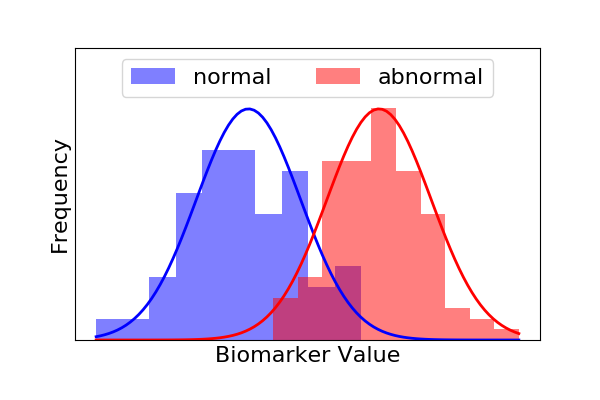
\includegraphics[height=3cm,trim=50 0 0 0, clip]{images/abnormal1.png}};
\node (mixModelLabel2) at (mixModel2.north) {Region 2};
\draw[->,line width=0.3mm] (tab1) -- (mixModel);

\node (tab2) at (3,0.25) {
\begin{tabular}{c | c | c | c}
& Patient 1 & Patient 2 & Patient 3\\
\hline
  Region 1 & \textcolor{green!60!black}{normal} & \textcolor{green!60!black}{normal} & \textcolor{red}{abnormal}\\
  Region 2 & \textcolor{green!60!black}{normal} & \textcolor{red}{abnormal} & \textcolor{red}{abnormal}\\ 
\end{tabular}
};
\draw[->,line width=0.3mm] (3,1.5) -- (tab2);

\node (seq) at (3,-1.5) {Estimated Sequence: Region 2 $\rightarrow$ Region 1};
\node (seqDummyUp) at (3,-1.3) {};
\draw[->,line width=0.3mm] (tab2) -- (seqDummyUp);


\end{tikzpicture}
\caption[Event-based model diagram]{Diagram showing the key concepts behind the event-based model. We assume a toy dataset (top-left) of two region-of-interest biomarkers from three patients, which are at different stages along a hypothetical disease progression timeline (bottom-left). The aim is to estimate which region became abnormal earlier in the disease process. The event-based model solves this by fitting a mixture model to the data (top-right), where the two distributions are assumed to represent normal and abnormal biomarker values respectively. The measurements from each patient are then assessed according to each distribution (middle-right). Finally, the sequence of abnormality is estimated from these values, by placing earlier in the sequence the regions/biomarkers for which there are more abnormal values in the dataset. Diagram made by me.}
\label{fig:bckEbmDiagram}
\end{figure}


The event-based model was introduced by Fonteijn et al. \cite{fonteijn2012event} in 2012 and describes the disease as a sequence of discrete events. A key diagram describing the EBM is given in Fig. \ref{fig:bckEbmDiagram}. Given a small dataset of biomarker measurements from subjects who are assumed to lie at unknown shifts along the disease progression timeline (X-axis), the EBM aims to estimate the order in which brain regions, or more generally any biomarker measurements, become abnormal as the disease progresses. The disease is modelled as a sequence of events, where each event represents a change in the patient state, such as the onset of a new symptom (e.g. 'patient shows a drop in cognitive performance') or measurement of tissue pathology (e.g. 'lumbar puncture shows reduced amyloid beta'). 

In section \ref{sec:ebm_theory} we present the theory behind the EBM, in section \ref{sec:model_est} we present the methods that are used to estimate the abnormality sequence, in section \ref{sec:mix_models} we show how to fit the mixture model parameters and in section \ref{sec:staging} we show how to stage the subjects using the EBM. 

\subsubsection{Theory}
\label{sec:ebm_theory}

The event-based model consists of a series of events $E_1, E_2, \dots , E_N$ and an ordering $S = [s(1), \dots, s(N)]$ which is a permutation of the integers $1,\dots, N$ creating the event ordering $E_{s(1)}, E_{s(2)},\dots, E_{s(N)}$. The set of events is specified a-priori.  Moreover, the model uses a dataset $X$ which contains a set of $X_i$ measurements for each subject $i$. These measurements $X_i$ are defined as $X_i = \{x_{i1}, x_{i2}, \dots, x_{iN}\}$, where $x_{ij}$ represents the value of biomarker $j$ in subject $i$ and is informative of event $E_j$ sin subject $i$. 

The event-based model makes two key assumptions: first, measurements are monotonic as the disease progresses and secondly, the event ordering is the same across all patients. The first assumption fits with the hypothetical model presented by Jack et al. \cite{jack2010hypothetical} in fig. \ref{fig:biomk_cascade}. Therefore, a patient for whom event $E_j$ has occurred cannot revert to a state where event $E_j$ did not occur. This assumption is essential because it ensures snapshots are informative about the event ordering \cite{fonteijn2012event}. The second assumption is necessary to be able to aggregate information about the event ordering from the entire set of subjects. 

The aim of the event-based model is to find the probability density function $p(S|X)$ of an event ordering given the biomarker data. One starts by fitting a model for the likelihood function $p(x_{ij}|E_j)$ the likelihood of measuring $x_{ij}$ given event $E_i$ occurred. A similar fit is obtained for $p(x_{ij}|\neg E_j)$, the likelihood of measuring $x_{ij}$ given event $E_j$ has not occurred. More information about mixture model fitting can be found in section \ref{sec:mix_models}. If a subject $i$ is at stage $k$ in the disease progression, events $E_{s(1)},\dots, E_{s(k)}$ have occurred while events $E_{s(k+1)},\dots, E_{s(N)}$ have not occurred. We can therefore define the likelihood of the data from subject $i$ given ordering $S$ as:

\begin{equation}
\label{eq:ebm1}
 p(X_i | S, k) = \prod_{j=1}^k p\left(x_{i,s(j)} | E_{s(j)} \right) \prod_{j=k+1}^N p\left(x_{i,s(j)} | \neg E_{s(j)}\right)
\end{equation}
 
where measurements $x_{ij}$ are assumed to be independent. Since the subject could potentially be at any stage $k$ in the progression, we integrate over $k$:

\begin{equation}
\label{eq:ebm2}
  p(X_i | S) = \sum_{k=0}^N p(k)p(X_i|S,k) 
\end{equation}

where $p(k)$ is the prior probability of the subject being at position $k$ in the sequence. A uniform prior is usually assumed here. Further assuming independence of measurements across patients we get:

\begin{equation}
\label{eq:ebm3}
 p(X|S) = \prod_{i=1}^P p(X_i | S)
\end{equation}

Combining equations \ref{eq:ebm1},\ref{eq:ebm2}, \ref{eq:ebm3} we get the total likelihood:

\begin{equation}
\label{eq:ebm4}
 p(X|S) = \prod_{i=1}^P \left[ \sum_{k=0}^N p(k) \left( \prod_{i=1}^k p\left(x_{i,s(j)} | E_{s(j)} \right) \prod_{i=k+1}^N p\left(x_{i,s(j)} | \neg E_{s(j)}\right) \right) \right]
\end{equation}

\subsubsection{Event Sequence Estimation}
\label{sec:model_est}

Applying Bayes' theorem  we can get the posterior on the sequence:

\begin{equation}
 p(S|X) = \frac{p(S)p(X|S)}{p(X)}
\end{equation}

As the marginal distribution $p(X)$ is analytically intractable, one uses a Markov-chain Monte Carlo (MCMC) algorithm to sample from the posterior distribution $p(S|X)$. One assumes flat priors on the sequence $S$ as any sequence could be equally likely. In the MCMC phase, at each iteration the sequence $S$ can be perturbed by swapping two randomly chosen events. This perturbation rule has been used by Fonteijn et al. \cite{fonteijn2012event}. However, another perturbation method used by Young et al. \cite{young2014data} randomly selects a source and target event and places the source event after the target event, sliding the other biomarkers accordingly (see Fig. \ref{fig:backgr_mcmc_perturb}). The resulting sequence $S^{new}$ is accepted with probability $p = min(1, a)$ where $ a = p(X|S^{new})/p(X|S)$. Otherwise the old sequence is stored and the process is repeated. As MCMC depends on accurate initialisation, one also runs a greedy ascent algorithm in order to find the sequence with the highest likelihood. The greedy ascent is very similar to the MCMC phase, the only difference being that $a$ is set to 1 if $p(X|S^{new}) > p(X|S)$ and to zero otherwise. Depending on the number of biomarkers, the greedy ascent is run for a few thousand iterations and repeated 10 times, with different random permutations of integers $1,\dots,N$ as the starting position. The maximum likelihood sequence obtained from greedy ascent is then used to initialise MCMC sampling, which usually runs for at least 100,000 iterations, again depending on problem size.

The resulting MCMC-sampled sequences are usually plotted in a positional variance matrix $M$ (Fig \ref{fig:bckEbmMcmc}), which is a compact way to represent uncertainty in the event ordering. Each element $M(i,j)$ represents the proportion of times event $E_{s(j)}$ appeared on position $i$ in the sampled sequences, given some \emph{master sequence} $S$. $S$ is usually set to be the maximum likelihood sequence or the \emph{characteristic ordering}, which is given by the average position of the events in the MCMC samples \cite{fonteijn2012event}.

\newcommand{\nodeRad}{0.4cm}

\begin{figure}
\centering
\begin{subfigure}[b]{0.45\textwidth}
 \centering
 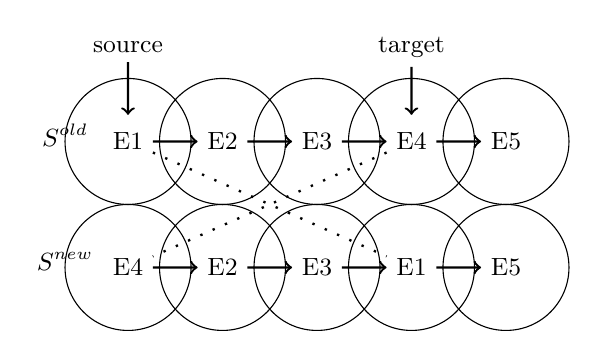
\begin{tikzpicture}[scale=0.8]
  \tikzstyle{every node}=[font=\small]


  \draw (-5,3) circle [radius=\nodeRad] node (E1) {E1};
  \draw (-3.5,3) circle [radius=\nodeRad] node (E2) {E2};  
  \draw (-2,3) circle [radius=\nodeRad] node (E3) {E3};
  \draw (-0.5,3) circle [radius=\nodeRad] node (E4) {E4};
  \draw (1,3) circle [radius=\nodeRad] node (E5) {E5};  
  \node (descold) at (-6,3.1) {$S^{old}$};
  \node (src) at (-5,4.5) {source};
  \node (trg) at (-0.5,4.5) {target};
  
  \draw[->,line width=0.3mm] (E1) -- (E2);
  \draw[->,line width=0.3mm] (E2) -- (E3);
  \draw[->,line width=0.3mm] (E3) -- (E4);
  \draw[->,line width=0.3mm] (E4) -- (E5);
  \draw[->,line width=0.3mm,shorten >=3pt] (src) -- (E1);
  \draw[->,line width=0.3mm,shorten >=3pt] (trg) -- (E4);  
  
  \draw (-5,1) circle [radius=\nodeRad] node (E4b) {E4};
  \draw (-3.5,1) circle [radius=\nodeRad] node (E2b) {E2};  
  \draw (-2,1) circle [radius=\nodeRad] node (E3b) {E3};
  \draw (-0.5,1) circle [radius=\nodeRad] node (E1b) {E1};
  \draw (1,1) circle [radius=\nodeRad] node (E5b) {E5};
  \node (descnew) at (-6,1.1) {$S^{new}$};
  
  \draw[->,line width=0.3mm] (E4b) -- (E2b);
  \draw[->,line width=0.3mm] (E2b) -- (E3b);
  \draw[->,line width=0.3mm] (E3b) -- (E1b);
  \draw[->,line width=0.3mm] (E1b) -- (E5b);
  
  \draw[loosely dotted, line width=0.3mm] (E1) -- (E1b);
  \draw[loosely dotted, line width=0.3mm] (E4) -- (E4b);  
 
  
\end{tikzpicture}
\caption{Fonteijn et al. \cite{fonteijn2012event}}
\end{subfigure}
%   ~
\begin{subfigure}[b]{0.45\textwidth}
 \centering
 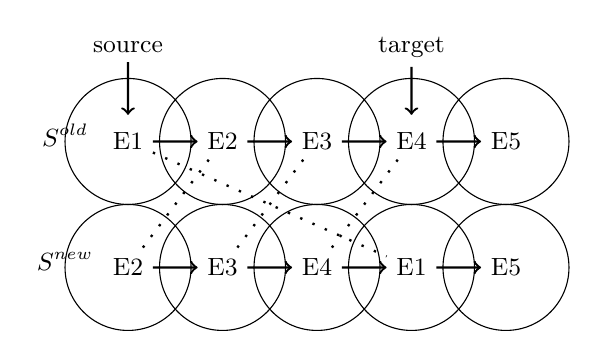
\begin{tikzpicture}[scale=0.8]
  \tikzstyle{every node}=[font=\small]


  \draw (-5,3) circle [radius=\nodeRad] node (E1) {E1};
  \draw (-3.5,3) circle [radius=\nodeRad] node (E2) {E2};  
  \draw (-2,3) circle [radius=\nodeRad] node (E3) {E3};
  \draw (-0.5,3) circle [radius=\nodeRad] node (E4) {E4};
  \draw (1,3) circle [radius=\nodeRad] node (E5) {E5};  
  \node (descold) at (-6,3.1) {$S^{old}$};
  \node (src) at (-5,4.5) {source};
  \node (trg) at (-0.5,4.5) {target};
  
  \draw[->,line width=0.3mm] (E1) -- (E2);
  \draw[->,line width=0.3mm] (E2) -- (E3);
  \draw[->,line width=0.3mm] (E3) -- (E4);
  \draw[->,line width=0.3mm] (E4) -- (E5);
  \draw[->,line width=0.3mm,shorten >=3pt] (src) -- (E1);
  \draw[->,line width=0.3mm,shorten >=3pt] (trg) -- (E4);  
  
  \draw (-5,1) circle [radius=\nodeRad] node (E2b) {E2};
  \draw (-3.5,1) circle [radius=\nodeRad] node (E3b) {E3};  
  \draw (-2,1) circle [radius=\nodeRad] node (E4b) {E4};
  \draw (-0.5,1) circle [radius=\nodeRad] node (E1b) {E1};
  \draw (1,1) circle [radius=\nodeRad] node (E5b) {E5};
  \node (descnew) at (-6,1.1) {$S^{new}$};
  
  \draw[->,line width=0.3mm] (E2b) -- (E3b);
  \draw[->,line width=0.3mm] (E3b) -- (E4b);
  \draw[->,line width=0.3mm] (E4b) -- (E1b);
  \draw[->,line width=0.3mm] (E1b) -- (E5b);
  
  \draw[loosely dotted, line width=0.3mm] (E1) -- (E1b);
  \draw[loosely dotted, line width=0.3mm] (E2) -- (E2b);
  \draw[loosely dotted, line width=0.3mm] (E3) -- (E3b);
  \draw[loosely dotted, line width=0.3mm] (E4) -- (E4b);
  
\end{tikzpicture}
\caption{Young et al. \cite{young2014data}}
\end{subfigure}

\caption[MCMC perturbation rules in the event-based model]{MCMC perturbation rules used by (a) Fonteijn et al. \cite{fonteijn2012event} and (b) Young et al. \cite{young2014data}. Both methods assume randomly selected source and target events. The method by Fonteijn et al. only swaps the source event (E1) with the target event (E4). On the other hand, the perturbation used by Young et al. moves a source event after a target event and slides the other biomarkers accordingly.  Diagram made by me.}
\label{fig:backgr_mcmc_perturb}
\end{figure}

\begin{figure}
\centering
\begin{tikzpicture}[scale = 0.8]
  \tikzstyle{every node}=[font=\small]

  \node (samples) at (-2.5,4) {\textbf{MCMC samples}};
  \draw (-5,3) circle [radius=\nodeRad] node (E2) {E2};
  \draw (-3.5,3) circle [radius=\nodeRad] node (E1) {E1};  
  \draw (-2,3) circle [radius=\nodeRad] node (E4) {E4};
  \draw (-0.5,3) circle [radius=\nodeRad] node (E3) {E3};
  
  \draw (-5,2) circle [radius=\nodeRad] node (E1m) {E1};
  \draw (-3.5,2) circle [radius=\nodeRad] node (E2m) {E2};  
  \draw (-2,2) circle [radius=\nodeRad] node (E4m) {E4};
  \draw (-0.5,2) circle [radius=\nodeRad] node (E3m) {E3};
  
  \draw (-5,0) circle [radius=\nodeRad] node (E2s) {E2};
  \draw (-3.5,0) circle [radius=\nodeRad] node (E1s) {E1};
  \draw (-2,0) circle [radius=\nodeRad] node (E3s) {E3};
  \draw (-0.5,0) circle [radius=\nodeRad] node (E4s) {E4};
  
  \node (1) at (-5.7,3) {1};
  \node (2) at (-5.7,2) {2};
  \node (T) at (-5.7,0) {T};
  
  \draw[loosely dotted, line width=0.3mm] (2) -- (T);
  
  
  \draw[->,line width=0.3mm] (E2) -- (E1);
  \draw[->,line width=0.3mm] (E1) -- (E4);
  \draw[->,line width=0.3mm] (E4) -- (E3);
  
  \draw[->,line width=0.3mm] (E1m) -- (E2m);
  \draw[->,line width=0.3mm] (E2m) -- (E4m);
  \draw[->,line width=0.3mm] (E4m) -- (E3m);
  
  \draw[->,line width=0.3mm] (E2s) -- (E1s);
  \draw[->,line width=0.3mm] (E1s) -- (E3s);
  \draw[->,line width=0.3mm] (E3s) -- (E4s);
  
  % characteristic ordering 
  
  \node (ordering) at (-2.5,-2) {\textbf{Maximum Likelihood Ordering}};
  \draw (-5,-3) circle [radius=\nodeRad] node (E2c) {E2};
  \draw (-3.5,-3) circle [radius=\nodeRad] node (E1c) {E1};  
  \draw (-2,-3) circle [radius=\nodeRad] node (E4c) {E4};
  \draw (-0.5,-3) circle [radius=\nodeRad] node (E3c) {E3};

  
  \draw[->,line width=0.3mm] (E2c) -- (E1c);
  \draw[->,line width=0.3mm] (E1c) -- (E4c);
  \draw[->,line width=0.3mm] (E4c) -- (E3c);
  
  \node (pic) at (5,0) {\includegraphics[scale=0.4]{../code/toyEBMs/figures/small5/posVarianceMatrix.pdf}};
  
  \draw (ordering.east) -| (1.5,0.3) -- (2.5,0.3);
  \draw (samples.east) -| (5.7,3);
  
  \draw (4,2.7) |- (7,3) -- (7,2.7);
  \draw (2.7,2) -| (2.5,-1.2) -- (2.7,-1.2);
  
\end{tikzpicture}
\caption[Event-based model - MCMC sampling diagram]{MCMC sampling and positional variance computation. MCMC sampling finds a series of $T$ samples, which are then used to derive the \emph{characteristic ordering}, where events are ordered according to their average position in the MCMC samples. Entries $M(i,j)$ in the positional variance matrix stores the relative number of times each event appeared in each position in the sequence. The events in the positional variance matrix are ordered according to the characteristic ordering.  Diagram made by me.}
\label{fig:bckEbmMcmc}
\end{figure}

\subsubsection{Mixture Models for Data Likelihood}
\label{sec:mix_models}

In equation \ref{eq:ebm1} we need to model the distributions $p\left(x_{i,j} | E_{j} \right)$ and $p\left(x_{i,j} | \neg E_{j}\right)$ of abnormal and normal biomarker values, using the measurements in $X$. Fonteijn et al. \cite{fonteijn2012event} used a Gaussian distribution for $p\left(x_{i,j} | \neg E_{j}\right)$ and a uniform distribution for $p\left(x_{i,j} | E_{j} \right)$. The parameters for the Gaussian distribution were set as the mean and standard deviation of biomarker values corresponding to controls, while the limits of the uniform distribution were set to be the minimum and maximum observed biomarker values. While this works in familial AD and Huntington's disease \cite{fonteijn2012event} due to well-defined control populations, this does not work well in sporadic AD due to the control population being not well-defined -- e.g. some controls can already have abnormal amyloid levels, which could result in the distribution for normal values encompassing all observed values. Therefore, the approach of Young et al. \cite{young2014data} for sporadic AD involved optimising the mixture model parameters based on the subjects' data in a data-driven manner. In this case, prior constraints were used on the mixture model parameters, i.e. the mean and standard deviation of the gaussian distributions, for biomarkers that did not change from healthy to diseased subjects.

\subsubsection{Patient Staging and Diagnosis Prediction}
\label{sec:staging}

After the maximum likelihood sequence has been found using the greedy ascent method described in section \ref{sec:model_est}, each subject can be assigned a disease stage $k$ as follows:

\begin{equation}
\label{eq:staging}
 k = \argmax_k p(k) p(X_i | S, k) = p(k) \prod_{i=1}^k p\left(x_{i,s(j)} | E_{s(j)} \right) \prod_{i=k+1}^N p\left(x_{i,s(j)} | \neg E_{s(j)}\right)
\end{equation}
 
As before, the prior $p(k)$ is assumed to be uniform. It should be noted that stages range from zero to $N$, the number of events. If a subject is at stage $k$ it means that all events up to and including $k$ have occurred while the events after $k$ have not occurred. 

The event-based model can also be used to classify subjects into controls and AD, or any other symptomatic subgroups \cite{young2014data}. Given a threshold stage $t$, one can predict all subjects having a stage less than or equal to $t$ to be controls and all subjects with stages greater than $t$ to be patients. The optimal threshold is the one which maximises the balanced accuracy, defined as follows:

\begin{equation}
 Accuracy = \frac{TP + TN}{TP + FP + FN + TN}
\end{equation}
where $TP$, $FP$, $FN$, $TN$ represent the number of true positive, false positive, false negative and true negative subjects respectively.

 
\subsubsection{Discussion}

The EBM is a useful tool for modelling the progression of diseases when only limited, cross-sectional data is available. The model can also be usd to stage subjects, in discreete units, along the disease progression timeline. The model parameters are estimated using Markov Chain Monte Carlo sampling, based on optimising a conditional likelihood. 

\subsubsection{Advantages and Limitations}

% Advantages
The event-based model by Fonteijn et al. \cite{fonteijn2012event} has several advantages. It is a data-driven progression model which does not use a-priori defined clinical stages, which can often be unreliable and can limit the temporal resolution of the model. Moreover, it does not require longitudinal data, which makes it very useful for analysing rare types of dementia for which comprehensive longitudinal datasets do not exist. The Bayesian framework in which it is formulated also allows it to estimate uncertainty in the abnormality sequence. The model can also easily combine data from different modalities.  

% Limitations
The current model has several limitations. The trajectory parameters are modelled as step functions, which is a strong assumption given the continuous nature many biomarkers used in AD. Secondly, in the fitting process the conditional probability of the sequence given a-priori estimated distribution parameters is optimised, instead of the joint distribution over the sequence and the distribution parameters, which can result in a suboptimal solution. Third, the model cannot use longitudinal biomarker  measurements in order to enable more precise staging and prognosis estimates.  Finally, the model also assumes that all subjects follow the same progression sequence, which is not the case in heterogeneous datasets due to differences in the underlying pathology, genetics and environmental factors. Identifiability can also be an issue, mostly when, for a certain biomarker, the distributions of normal and abnormal values overlap -- this can result in the biomarker's event being placed either towards the beginning or the end of the sequence, even if the true position of that event is in the middle of the sequence.


\subsection{Differential Equation Model}
\label{sec:bckDem}


\begin{figure}[h]
 \centering
 
 \par{\huge $\xRightarrow{\text{Forward Model}}$}
 
 \begin{subfigure}{0.3\textwidth}
    \centering
    What we want\\
    \vspace{1em}
    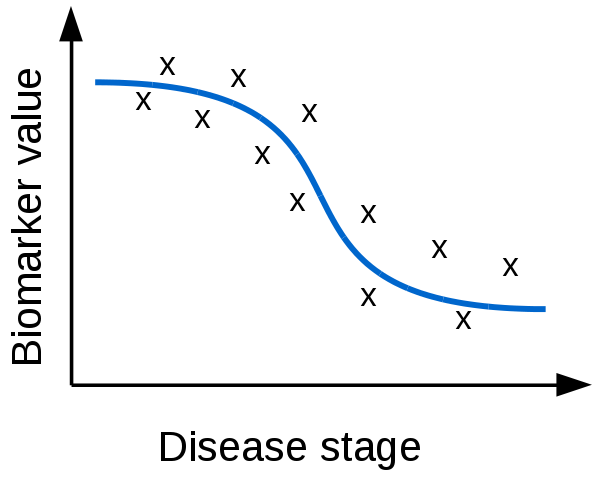
\includegraphics[width=0.90\textwidth]{images/demNewFigs/fig1.png}
%     \caption{}
    \vspace{1em}
 \end{subfigure}
 \begin{subfigure}{0.3\textwidth}
     \centering
     \vspace{1em}
     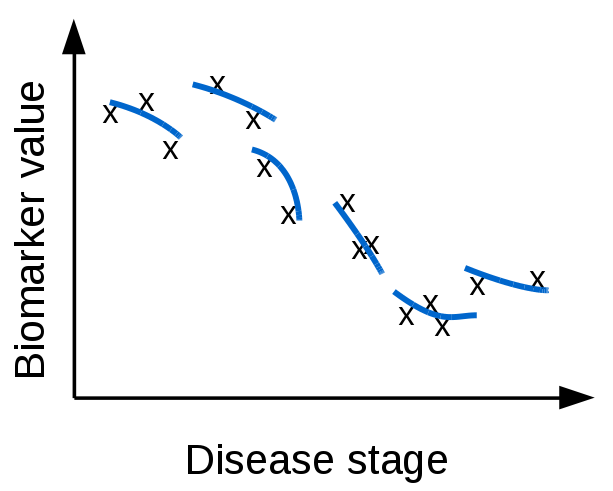
\includegraphics[width=\textwidth]{images/demNewFigs/fig2.png}
%      \caption{}
     \vspace{1em}
 \end{subfigure}
 \begin{subfigure}{0.3\textwidth}
     \centering
     What we have\\
     \vspace{1em}
     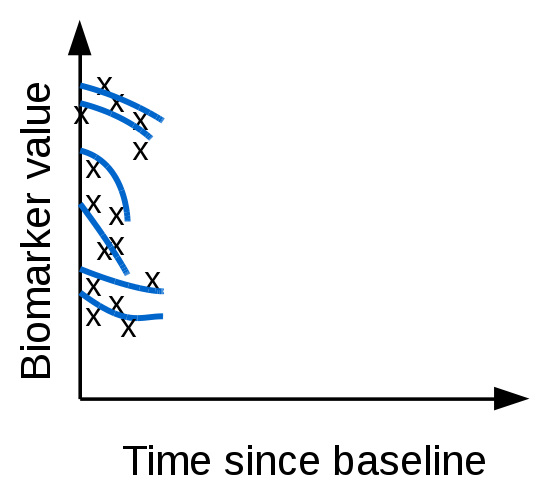
\includegraphics[width=0.90\textwidth,trim= 0 0 0 30]{images/demNewFigs/fig3.png}
%      \caption{}
     \vspace{1em}
 \end{subfigure}
 
 \begin{subfigure}{0.34\textwidth}
    \centering
    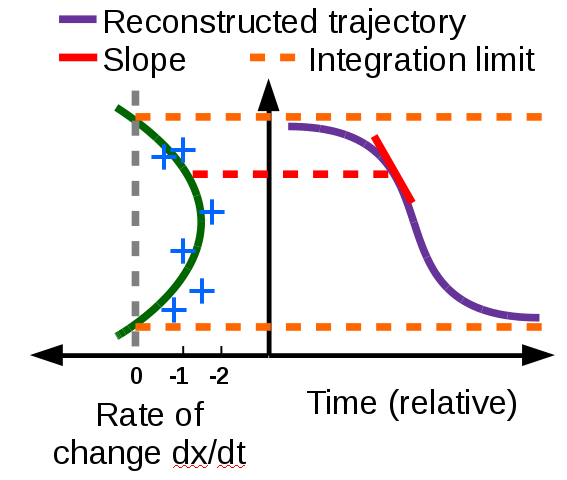
\includegraphics[width=\textwidth]{images/demNewFigs/fig5.png}
%     \caption{}
    \vspace{1em}
 \end{subfigure}
  \begin{subfigure}{0.3\textwidth}
  \centering
  \vspace{-3.5em}
  $$
  lim_{\Delta t \xrightarrow{}  0} \frac{\Delta x}{\Delta t} = \frac{\delta x}{\delta t} = f(x)
  $$
  
  Solve for $x$ using the Euler method:
  \begin{align*}
  t_1 &= t_0 + \delta t \\
  x_1 &= x_0 + f(x_0) \delta t \label{eq:dem3}
  \end{align*}
 \end{subfigure}
%\hspace{12em}
 \begin{subfigure}{0.3\textwidth}
     \centering
     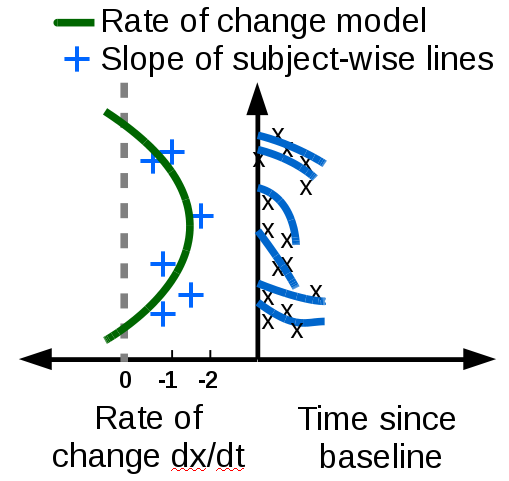
\includegraphics[width=\textwidth]{images/demNewFigs/fig4.png}
%      \caption{}
     \vspace{1em}
 \end{subfigure}
 \vspace{-2em}
 \par{\huge $\xLeftarrow[\text{Inverse Problem}]{}$}
 
 \caption[Diagram of the Differential Equation Model (DEM)]{Diagram of the Differential Equation Model (DEM). (top-left) Hypothetical biomarker signature that needs to be reconstructed, along with subject measurements. (top-middle) To make the model more realistic, each subject is made to follow a slightly different trajectory due to heterogeneity. (top-right) In practice, we don't know the disease stage, so we align the measurements at time since baseline visit. (bottom-right) The DEM model estimates a rate of change model from the slopes of lines fitted to each subject's biomarker data. At least two measurements per subject are required in order to estimate this slope. (top-middle) The DEM then performs a line integral using the Euler method to recover the biomarker trajectory (top-right).  Diagram made by me.}
\label{fig:bckDEM}
\end{figure}

The differential equation model (DEM) \cite{ashford2001modeling, yang2011quantifying, sabuncu2011dynamics, villemagne2013amyloid, oxtoby2018} constructs the biomarker trajectories from the change in biomarker values between different visits (Fig \ref{fig:bckDEM}). In many medical settings we only have short-term longitudinal data, hence the biomarker scores $s$ are observed for each subject over a few visits. By determining how these scores change ($\Delta s$) over time ($t$) during a specified time interval $\Delta t$, the temporal rate of progression ($\Delta s/\Delta t$) can be modelled as a function of the mean biomarker value $f(s)$ \cite{ashford2001modeling}:

\begin{equation}
\label{eq:dem_1}
 \frac{\Delta s}{\Delta t} \approx f(s)
\end{equation}

The model given by $f(s)$ can be parametric (e.g. linear, polynomial) or non-parametric such as Gaussian Processes (GP). We then perform a line integral along $f(s)$ to recover $s(t)$. More explicitly, if we take the limit as $\Delta t \xrightarrow{} 0$ from Eq. \ref{eq:dem_1}, we get that:

\begin{equation}
\label{eq:dem2}
lim_{\Delta t \xrightarrow{}  0} \frac{\Delta s}{\Delta t} = \frac{\delta s}{\delta t} = f(s)
\end{equation}

Solving this numerically is done using the Euler method. We set an initial $(t_0,s_0)$ and small increment step $\delta t$ and find the next pair $(t_1, s_1)$ as follows:

\newcommand\numberthis{\addtocounter{equation}{1}\tag{\theequation}}

\begin{align*}
 t_1 &= t_0 + \delta t \\
 s_1 &= s_0 + f(s_0) \delta t \numberthis \label{eq:dem3}
\end{align*}

This is repeated until the full curve defined by $(t_0, s_0), (t_1, s_1), \dots, (t_n, s_n)$ is reconstructed. Since the DEM model is univariate, the process is repeated independently for the other biomarkers. 

\subsubsection{Advantages and Limitations}

The differential equation model has several advantages. It is a fully data-driven method that does not require a-priori defined clinical categories. In contrast to the event-based model, it can estimate non-parametric biomarker trajectories which make minimal assumptions on the shape of the biomarker trajectories. Moreover, the DEM can use any model to estimate the change in biomarker values. While \cite{oxtoby2018} used Gaussian Processes to estimate the change in values, others \cite{villemagne2013amyloid} used polynomial functions.

The model has several limitations. First of all, the DEM is univariate, so the biomarker trajectories are fit independently. This requires alignment on the temporal axis after they are recovered, and makes it susceptible to noise within that biomarker\footnote{A multivariate model would've been able to use information from other biomarkers to help estimate such a noisy trajectory, hence are more robust in theory.}. Secondly, in this formulation the model does not allow one to directly estimate uncertainty in the trajectory values along the y-axis. One option for estimating uncertainty is to integrate posterior samples of the differential model and then align them all on the temporal axis. However, this does not result in true confidence intervals, since at the anchor point there will be zero uncertainty.


\subsection{The Disease Progression Score Model}
\label{sec:bckDps}

\begin{figure}
\centering
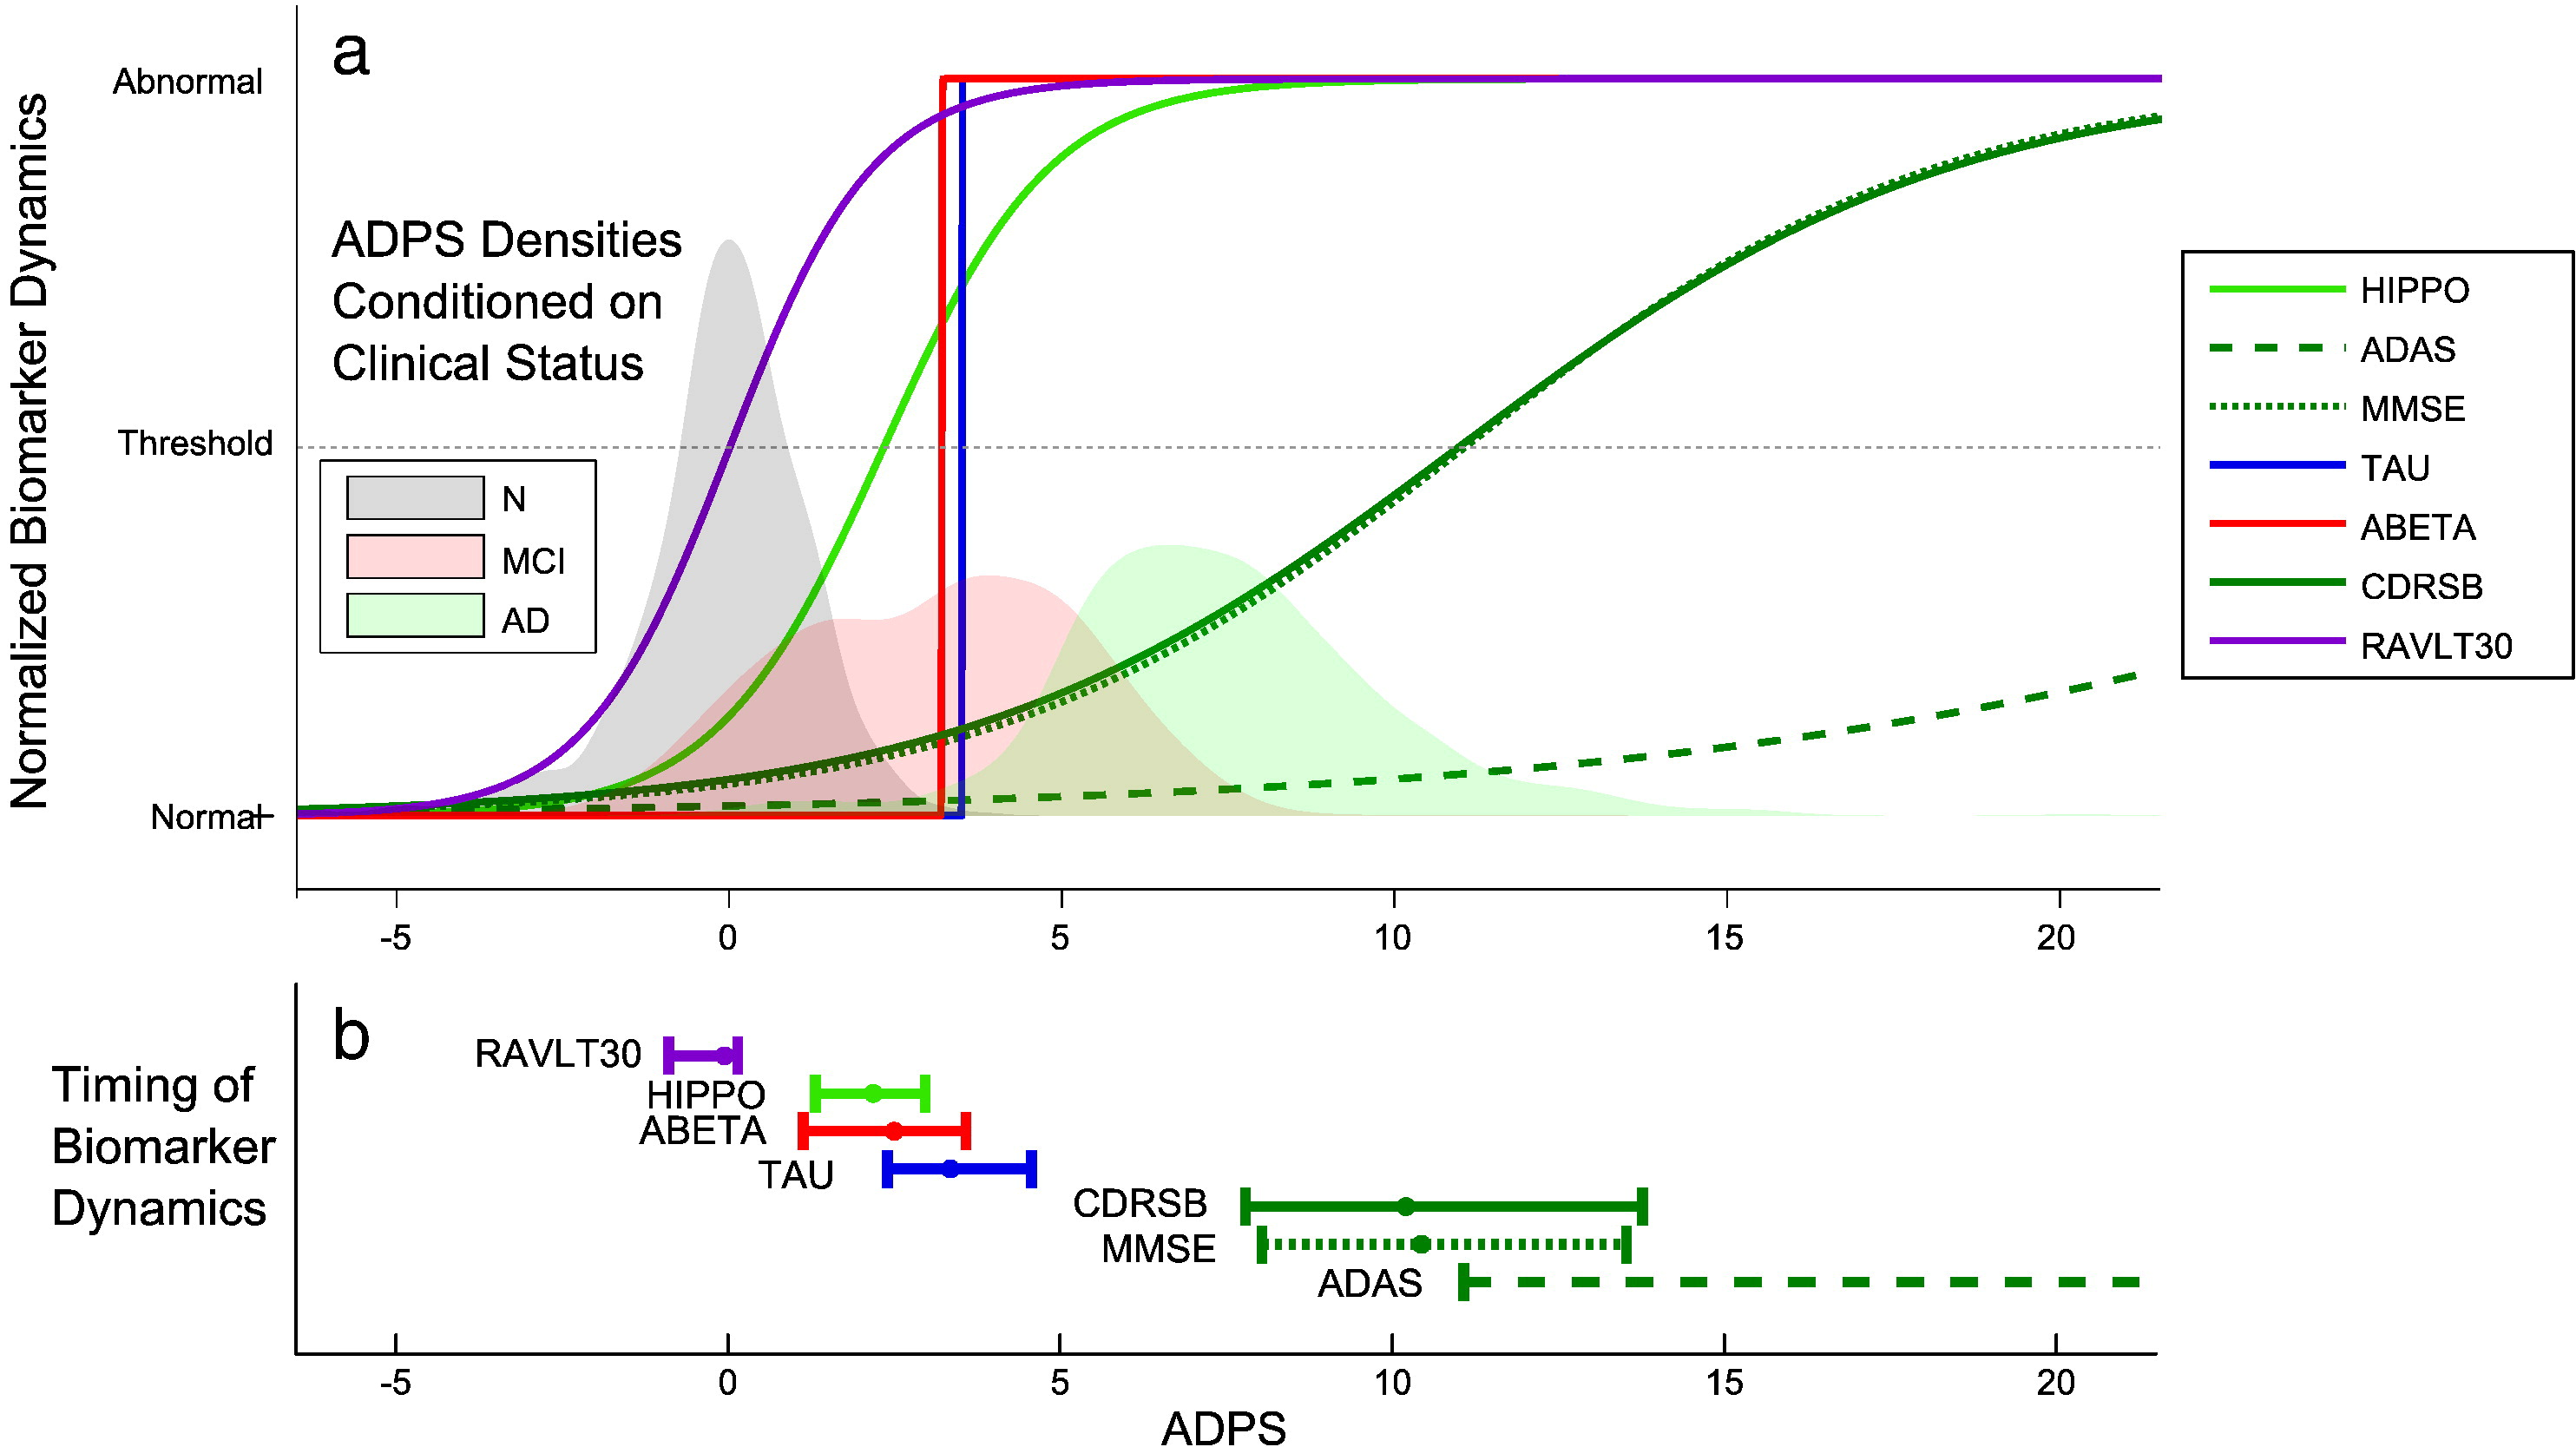
\includegraphics[width=\textwidth]{images/jedynakDiag}
\caption[ADNI biomarker trajectories estimated by Jedynak et al. \cite{jedynak2012computational}]{Biomarker trajectories estimated by the disease progression model by Jedynak et al. \cite{jedynak2012computational}. Reproduced with permission from \cite{jedynak2012computational}.}
\label{fig:bckDps}
\end{figure}

The disease progression score (DPS) model was proposed by Jedynak et al. \cite{jedynak2012computational}. It is based on three main assumptions:
\begin{itemize}
 \item Subjects follow a common disease progression but they have a different age at onset and progression speed.
 \item Each biomarker trajectory is a monotonic curve that follows a sigmoidal shape
 \item The speed of progression of each subject is the same across the entire disease time-course.
\end{itemize}

Biomarker trajectories estimated by the model for typical AD progression are shown in Fig. \ref{fig:bckDps}. The model estimates the optimal shape\footnote{within a parametric family, in this case sigmoidal family} of the biomarker trajectories, while estimating a disease progression score for each subject, which is the stage along the disease time course. The disease progression score $s_{ij}$ for subject $i$ at visit $j$ is defined as a linear transformation of age $t_{ij}$:

\begin{equation}
\label{eq:dps}
 s_{ij} = \alpha_i t_{ij} + \beta_i
\end{equation}
% sigmoidal functions
where $\alpha_i$ and $\beta_i$ represent the speed of progression and time shift (i.e. disease onset) of subject $i$. 

The DPS model assumes that biomarker measurements are independent and follow a sigmoidal trajectory $f(s)$ given the disease progression score $s$. The sigmoidal function for biomarker $k$ with parameters $\theta_k = [a_k,b_k,c_k,d_k]$ is defined as:

\begin{equation}
 f(s;\theta_k) = \frac{a_k}{1+exp(-b_k(s-c_k))} + d_k
\end{equation}
where $d_k$ is the minimum value, $d_k+a_k$ is the maximum value, $a_kb_k/4$ is the maximum slope and $c_k$ is the inflexion point. Authors choose to model the biomarker trajectory as parametric sigmoidal curves because they provide a better fit than linear models \cite{sabuncu2011dynamics, caroli2010dynamics}, and can account for floor and ceiling effects. The value $y_{ijk}$ of biomarker $k$ from subject $i$ at visit $j$ is a normally distributed random variable:
\begin{equation}
 p(y_{ijk} | \alpha_i, \beta_i, \theta_k, \sigma_k) = N(y_{ijk} | f(\alpha_i t_{ij} + \beta_i; \theta_k), \sigma_k )
\end{equation}
We further define $I$ to be the set of all triplets $(i,j,k)$ for which measurements are available. Assuming independence across all measurements, we get the following model conditional likelihood:
\begin{equation}
 p(y | \alpha, \beta, \theta, \sigma) = \prod_{(i,j,k) \in I} p(y_{ijk} | \alpha_i, \beta_i, \theta_k, \sigma_k)
\end{equation}
where $y = [y_{ijk}]$ for $(i,j,k) \in I$. Vectors $\alpha = [\alpha_1, \dots, \alpha_S]$ and $\beta = [\beta_1, \dots, \beta_S]$, where $S$ is the number of subjects, denote the stacked parameters for the subject shifts. Vectors $\theta = [\theta_1, \dots, \theta_K]$ and $\sigma = [\sigma_1, \dots, \sigma_K]$, with $K$ being the number of biomarkers, represent the stacked parameters for the sigmoidal trajectories and measurement noise specific to each biomarker.

The parameters of the model are therefore $\Theta = [\alpha, \beta, \theta, \sigma]$ and the log-likelihood function associated with it is:
\begin{equation}
 l(\alpha, \beta, \theta, \sigma) = \sum_{(i,j,k) \in I} log \sigma_k + \frac{1}{2 \sigma_k ^2} \left( y_{ijk} - f(\alpha_i t_{ij})\right)
\end{equation}

\subsubsection{Model Fitting}

Model fitting is done by loopy belief propagation, which alternates between optimising the sigmoidal parameters $\sigma$ and the subject specific parameters $\alpha, \beta$. Alg. \ref{fig:algo_dps} shows the fitting procedure. In line \ref{alg:init}, we initialise $\alpha_i = 1$, $\beta_i = 0$ for every $i$. On lines \ref{alg:theta} and \ref{alg:sigma} the optimal parameters for every biomarker trajectory are optimised. On line \ref{alg:alpha}, the subject specific shifts and progression speeds are also optimised. On line \ref{alg:identif}, a transformation is performed in order to make the model identifiable. For a similar reason, parameters $\alpha_i$ and $\beta_i$ are rescaled for every subject (line \ref{alg:rescale}), so that the disease progression scores of healthy controls have a mean $\mu_N$ of 0 and a standard deviation $\sigma_N$ of 1.

\begin{algorithm}
%  \KwData{this text}
%  \KwResult{how to write algorithm with \LaTeX2e }
 Initialise $\alpha^{(0)}$, $\beta^{(0)}$\;\label{alg:init}
 \For{$l=1$ to $L$}{
    \For{$k=1$ to $K$}{
      $\theta_k^{(1)} = \argmin_{\theta_k} \sum_{(i,j) \in I_k} (y_{ijk} - f(\alpha_i^{(0)} t_{ij} + \beta_i^{(0)} | \theta_k))^2$\label{alg:theta}\\
      $\sigma_k^{(1)^2} = \frac{1}{|I_k-2I-4|} \sum_{(i,j) \in I_k} (y_{ijk} - f(\alpha_i^{(0)} t_{ij} + \beta_i^{(0)} | \theta_k))^2$\label{alg:sigma}
    }
    \For{$i=1$ to $I$}{
      $\alpha_i^{(1)}, \beta_i^{(1)} = \argmin_{\alpha_i, \beta_i}  \sum_{(j,k) \in I_i} \frac{1}{\sigma_k^{(1)^2}}(y_{ijk} - f(\alpha_i t_{ij} + \beta_i | \theta_k^{(1)}))^2$\label{alg:alpha}
    }
    $\alpha^{(0)}=\alpha^{(1)}, \beta^{(0)}=\beta^{(1)}$\label{alg:update}
 }

  \For{$k=1$ to $K$}{
    \If{$b_k < 0$}{
      $a_k^{(1)} = -a_k^{(1)}, b_k^{(1)} = -b_k^{(1)}, d_k^{(1)} = d_k^{(1)}+a_k^{(1)}$\label{alg:identif}\\
    }
  }
  
  \For{$i=1$ to $I$}{
    $\alpha_i = \frac{\alpha_i}{\sigma_N}, \beta_i = \frac{\beta_i - \mu_N}{\sigma_N}$\label{alg:rescale}
  }
 \caption{The optimisation procedure for the disease progression score by \cite{jedynak2012computational}.}
 \label{fig:algo_dps}
\end{algorithm}


\subsubsection{Advantages and Limitations}

The model by Jedynak et al. \cite{jedynak2012computational} has several advantages. As opposed to the differential equation model, the model is multivariate and automatically aligns biomarker trajectories on the same temporal axis. Furthermore, compared to the event-based model by \cite{fonteijn2012event}, the biomarker trajectories are modelled as continuous sigmoidal trajectories instead of step functions. Moreover, each subject has an associated time shift and progression speed. Parameter estimation is performed with loopy belief propagation which is very similar to the Expectation-Maximisation framework \cite{bishop2007pattern}, but using hard assignments of the latent variables at each iteration.

The model has several limitations. The main limitation of this model is that the trajectories are assumed to be sigmoidal, which is not necessarily the case for many biomarkers such as cognitive tests, which show continuous decline even in late stages of the disease. Furthermore, each subject is assumed to follow the same progression pattern, which is not true in many heterogeneous datasets such as ADNI. The DPS model can also suffer identifiability issues when it attempts to stage very early-stage or late-stage subjects, as in these time-windows the biomarker trajectories are mostly flat. This issue can generally be addressed by setting priors on the time-shift and progression-speed of the subjets.

\subsection{The Self-Modelling Regression Model}
\label{sec:bckSem}

\begin{figure}
\centering
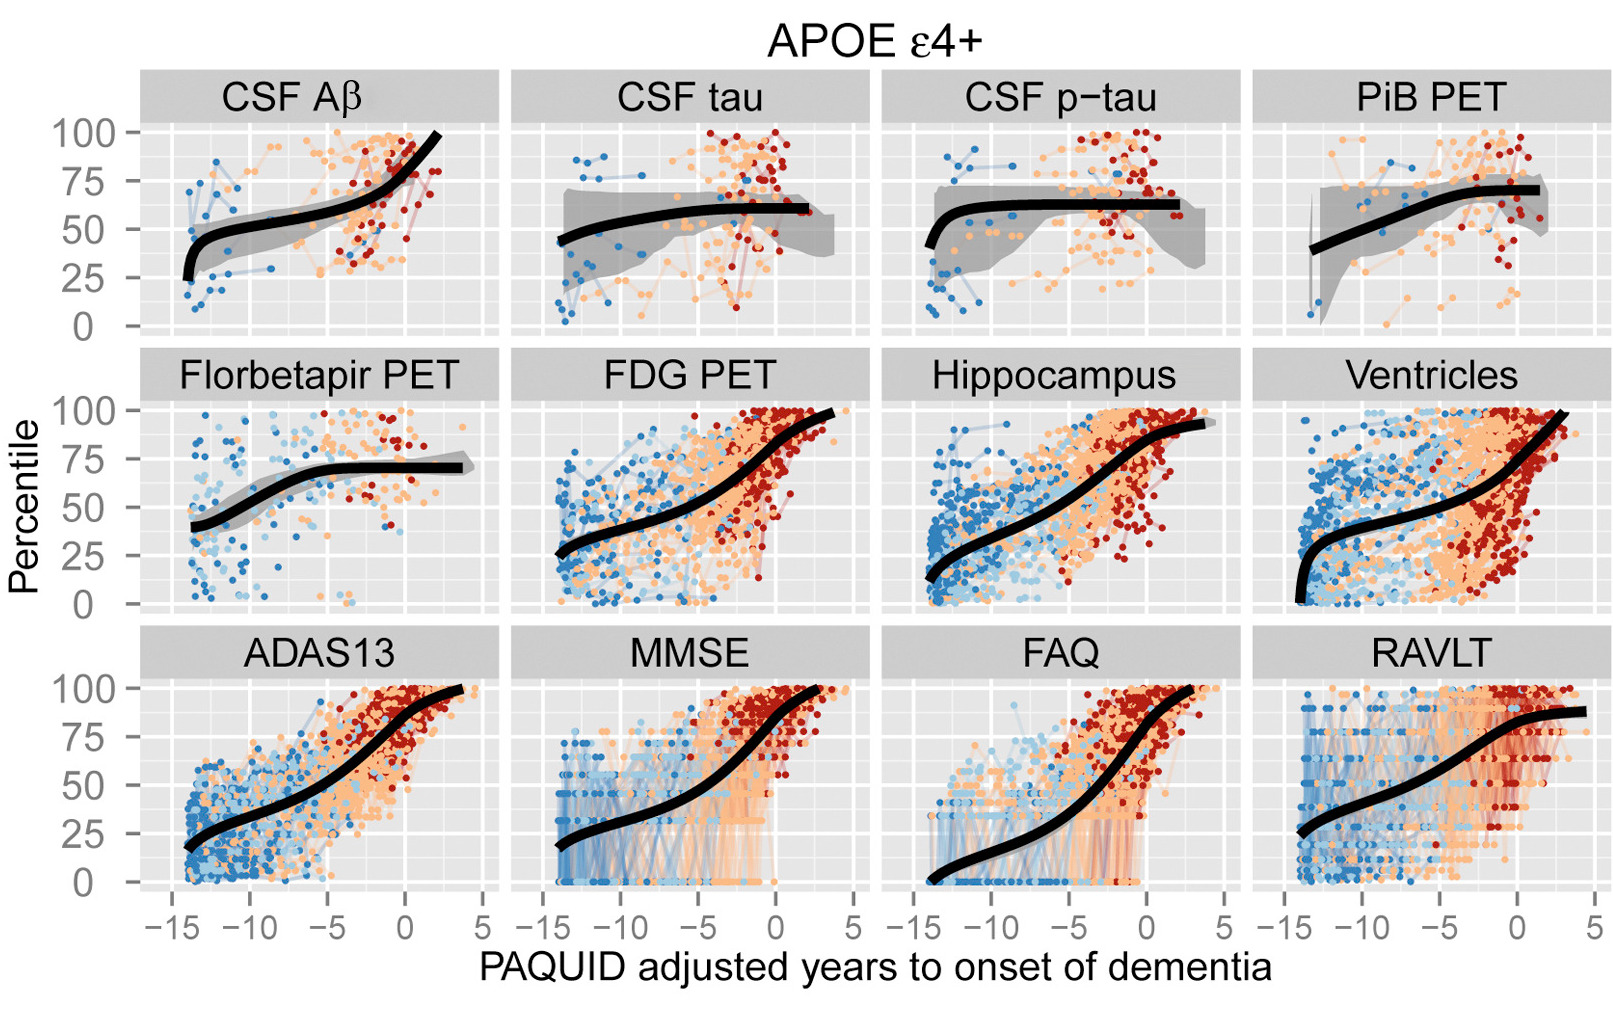
\includegraphics[width=0.9\textwidth]{images/semor_diagram_cropped}
\caption[ADNI Biomarker trajectories estimated by Donohue et al. \cite{donohue2014estimating}]{Biomarker trajectories estimated using the self-modelling regression approach by \cite{donohue2014estimating}. Reproduced with permission from \cite{donohue2014estimating}.}
\label{fig:bckSem}
\end{figure}

Self-modelling regression (SEMOR) is a method that fits several curves under the assumption of a common shape \cite{donohue2014estimating}. This approach has been used by Donohue et al. \cite{donohue2014estimating} to estimate non-parametric biomarker trajectories with linear subject-specific effects (Fig \ref{fig:bckSem}). Compared to the model by Jedynak et al. \cite{jedynak2012computational}, this model estimates non-parametric biomarker trajectories as fixed effects and includes subject-specific random effects. No subject-specific progression speed is modelled in the original formulation \cite{donohue2014estimating}. 

We assume that $Y_{ij}$ is the measurement of biomarker $j$ in subject $i$, $g_j$ is a continuously differentiable monotone function, $\gamma_i \sim N(0, \sigma_{\gamma}^2)$ is the time shift for subject $i$. The model is defined as follows:
\begin{equation}
 \label{eq:semor1}
 Y_{ij}(t) = g_j(t +\gamma_i)+\alpha_{0ij} + \alpha_{1ij}t+\epsilon_{ij}(t)
\end{equation}
where parameters $\alpha_{0ij}, \alpha_{1ij} \sim N(0, \Sigma_j)$ model a linear perturbation of the non-parametric trajectory $g_j$ for subject $i$ and biomarker $j$, $t$ is the time and $\epsilon_{ij}(t) \sim N(0, \sigma_j)$ is the measurement noise.  

\subsubsection{Parameter Fitting}

Fitting the model is also done by loopy belief propagation -- one iteratively estimates each set of parameters $(g_j, \gamma_i, \alpha)$ until convergence of the Residual Sum of Squares (RSS). The algorithm makes use of the following residuals:
\begin{equation}
\begin{cases}
  R_{ij}^g(t) = Y_{ij}(t) - \alpha_{0ij} - \alpha_{1ij}t & \qquad E\left[ R_{ij}^g(t) | g_j, t, \gamma_i \right] = g_j(t+\gamma_i)\\
  R_{ij}^{\alpha}(t) = Y_{ij}(t) - g_j(t+\gamma_i) & \qquad E\left[ R_{ij}^{\alpha}(t) | \alpha_{0ij}, \alpha_{1ij}, t \right] = \alpha_{0ij} + \alpha_{1ij}t\\
  R_{ij}^{\gamma}(t) = t-g_j^{-1}(Y_{ij}(t)) & \qquad E\left[ R_{ij}^{\gamma}(t) | \gamma_i \right] \approx g_j^{-1}(g_j(t+\gamma_i))-t = \gamma_i\\  
\end{cases}  
\end{equation}

Using the above residuals, the model is fit by initialising $\gamma_i$ and iterating the following steps\cite{donohue2014estimating}:
\begin{enumerate}
 \item Given $\gamma_i$, estimate $g_j$ by setting $\alpha_{0ij} = \alpha_{1ij} = 0$ and iterating the following subroutine:
 \begin{enumerate}
  \item Estimate $g_j$ by a monotone curve fit on $R_{ij}^g(t)$
  \item Estimate $\alpha_{0ij}, \alpha_{1ij}$ using the linear mixed model of $R_{ij}^{\alpha}(t)$. Repeat steps a and b until convergence of each $RSS_j = \sum_{it} \left[ Y_{ij}(t)-g_j(t+\gamma_i)-\alpha_{0ij}-\alpha_{1ij}t \right]^2 $
 \end{enumerate}
 
 \item Given the estimated $g_j$, set $\alpha_{0ij} = \alpha_{1ij} = \epsilon_{ij}(t) = 0$ and estimate each $\gamma_i$ with the average of $R_{ij}$ over all $j$ and $t$. Steps 1 and 2 are repeated until convergence of the total $RSS = \sum_{ijt} \left[ Y_{ij}(t)-g_j(t+\gamma_i)-\alpha_{0ij}-\alpha_{1ij}t \right]^2 $

\end{enumerate}

\subsubsection{Advantages and limitations}

The SEMOR model by \cite{donohue2014estimating} has many advantages. It robustly estimates biomarker trajectories using non-parametric curves, in contrast with previous approaches \cite{jedynak2012computational, fonteijn2012event}. Moreover, it also models unique trajectories for each subject as linear deviations from the average trajectories using a mixed effects model. Each subject also has it's own temporal shift along the disease progression timeline. Parameter estimation is done with loopy belief propagation, carefully alternating the optimisation of certain groups of parameters in order to minimise the residual of the cost function.

The model has some limitations. In its basic formulation it does not model different progression speeds for different individuals. Moreover, estimating all the subject-specific parameters $(\alpha_{0ij}, \alpha_{1ij}, \gamma_i)$ requires suitable priors and at least two longitudinal measurements per subject, which might not be available in some datasets. The high number of parameters that need to be estimated, especially the subject-specific parameters, can result in overfitting of the data, although this is mitigated to some extent by the priors placed on these parameters. Moreover, it also assumes that biomarker measurements are independent, which makes it unsuitable for modelling large sets of correlated biomarkers such as voxelwise measurements. Identifiability can also be an issue with the SEMOR model when the population trajectory becomes almost linear, such as in the case of biomarkers that don't show differences between healthy subejcts and patients.

\subsection{The Manifold-based Mixed Effects Model}
\label{sec:bckMan}

The manifold-based mixed effects model was introduced by Schiratti et al. in 2015 \cite{schiratti2015mixed}. The model generalises a previous linear mixed effects model by \cite{datar2012mixed} to account for time shifts and describes it in a Riemannian manifold setting. Each subject $i$ is assumed to have a trajectory $\gamma_{i}$ which is a deviation from the average population trajectory $\gamma$. The deviation is modelled as a time shift $\tau_i$ and progression speed $\alpha_i$ of subject $i$ along the disease timecourse. 

Let us assume we observe $p$ individuals, each having $n_i$ observations obtained at times $t_{i,1} < \dots < t_{i,n_i}$, each having $y_{i,1}, \dots, y_{i,n_i}$ biomarker measurements. For a geodesic $M$ and a point $p_0 \in M$ at time $t_0$ with velocity $v_0 \in T_{p_0}M$, we define $\gamma_{p_0,t_0,v_0} = Exp_{t_0,p_0}(\alpha_iv_0)(.)$ as the geodesic which passes through point $p_0$ at time $t_0$ with velocity $v_0$\footnote{In Riemannian geometry, $Exp$ refers to the exponential map, which is a function from the tangent space $T_{p}M$ into $M$ itself.}. We also consider $t_{i,j}$ and $y_{i,j}$ as the age and biomarker measurement for subject $i$ at visit $j$. This gives us the following model:

\begin{equation}
\label{eq:manifold1}
 y_{i,j} = Exp_{t_0+\tau_i,p_0}(\alpha_iv_0)(t_i,j) + \epsilon_{i,j}
\end{equation}
where
\begin{equation}
\label{eq:manifold2}
\begin{cases}
  \alpha_i = exp(\eta_i),\ \eta_i \sim \bigotimes_{i=1}^p N(0, \sigma_{\eta}^2)\\
    
  \tau_i \sim \bigotimes_{i=1}^p N(0, \sigma_{\tau}^2)\\  
  \epsilon_{i,j} \sim \bigotimes_{i,j} N(0, \sigma^2)\\  
\end{cases}
\end{equation}
The model assumes that each $\eta_i$ and $\tau_i$ are independent. The parameters of the model are $\theta = [p_0, t_0, v_0, \sigma_{\eta}, \sigma_{\tau}, \sigma]$. The model above can be re-written as:
\begin{align*}
  y_{i,j} &= \gamma_{p_0,t_0,v_0}(\alpha_iv_0(t_{i,j}-t_0-\tau_i))+\epsilon_{i,j}\\
          &= \gamma_i(t_{i,j})+\epsilon_{i,j} \numberthis \label{eq:manifold3}
\end{align*}
where $\gamma_i$ is the subject specific trajectory that is modelled as an affine reparametrisation of the average trajectory $\gamma_{p_0,t_0,v_0}$. The model described here is univariate. However, an extension of the model has been published by Schiratti et al. \cite{schiratti2015learning} which extends this framework to a multivariate analysis. 

Parameter estimation in the model by Schiratti et al. \cite{schiratti2015mixed} is performed using maximum likelihood estimation (MLE) using the Gauss-Hermite quadrature approximation, which is equivalent to the Laplace approximation of the observed likelihood. Authors used the Nelder-Mead method for estimating the numerical optimisation.


\subsubsection{Advantages and Limitations}

The model has several strengths and weaknesses. The main strength lies in the flexible Riemannian manifold framework, that allows one to create different models depending on how the inner product is defined. Moreover, the model estimates subject specific trajectories $\gamma_i$, time shifts $\tau_i$ and progression speeds $\alpha_i$. However, one of the limitations of the model is that it assumes a parametric form of the biomarker trajectories (i.e. sigmoidal).

\section{Spatiotemporal Disease Progression Models}
\label{sec:bckSpa}

Spatiotemporal models of disease progression have been proposed over the last few years. In the following section, we will present two key spatiotemporal models of progression that estimate voxelwise patterns of pathology, while also estimating latent subject-specific time shifts.

\subsection{The Voxelwise Disease Progression Model}
\label{sec:bckVox}


\begin{figure}
\centering
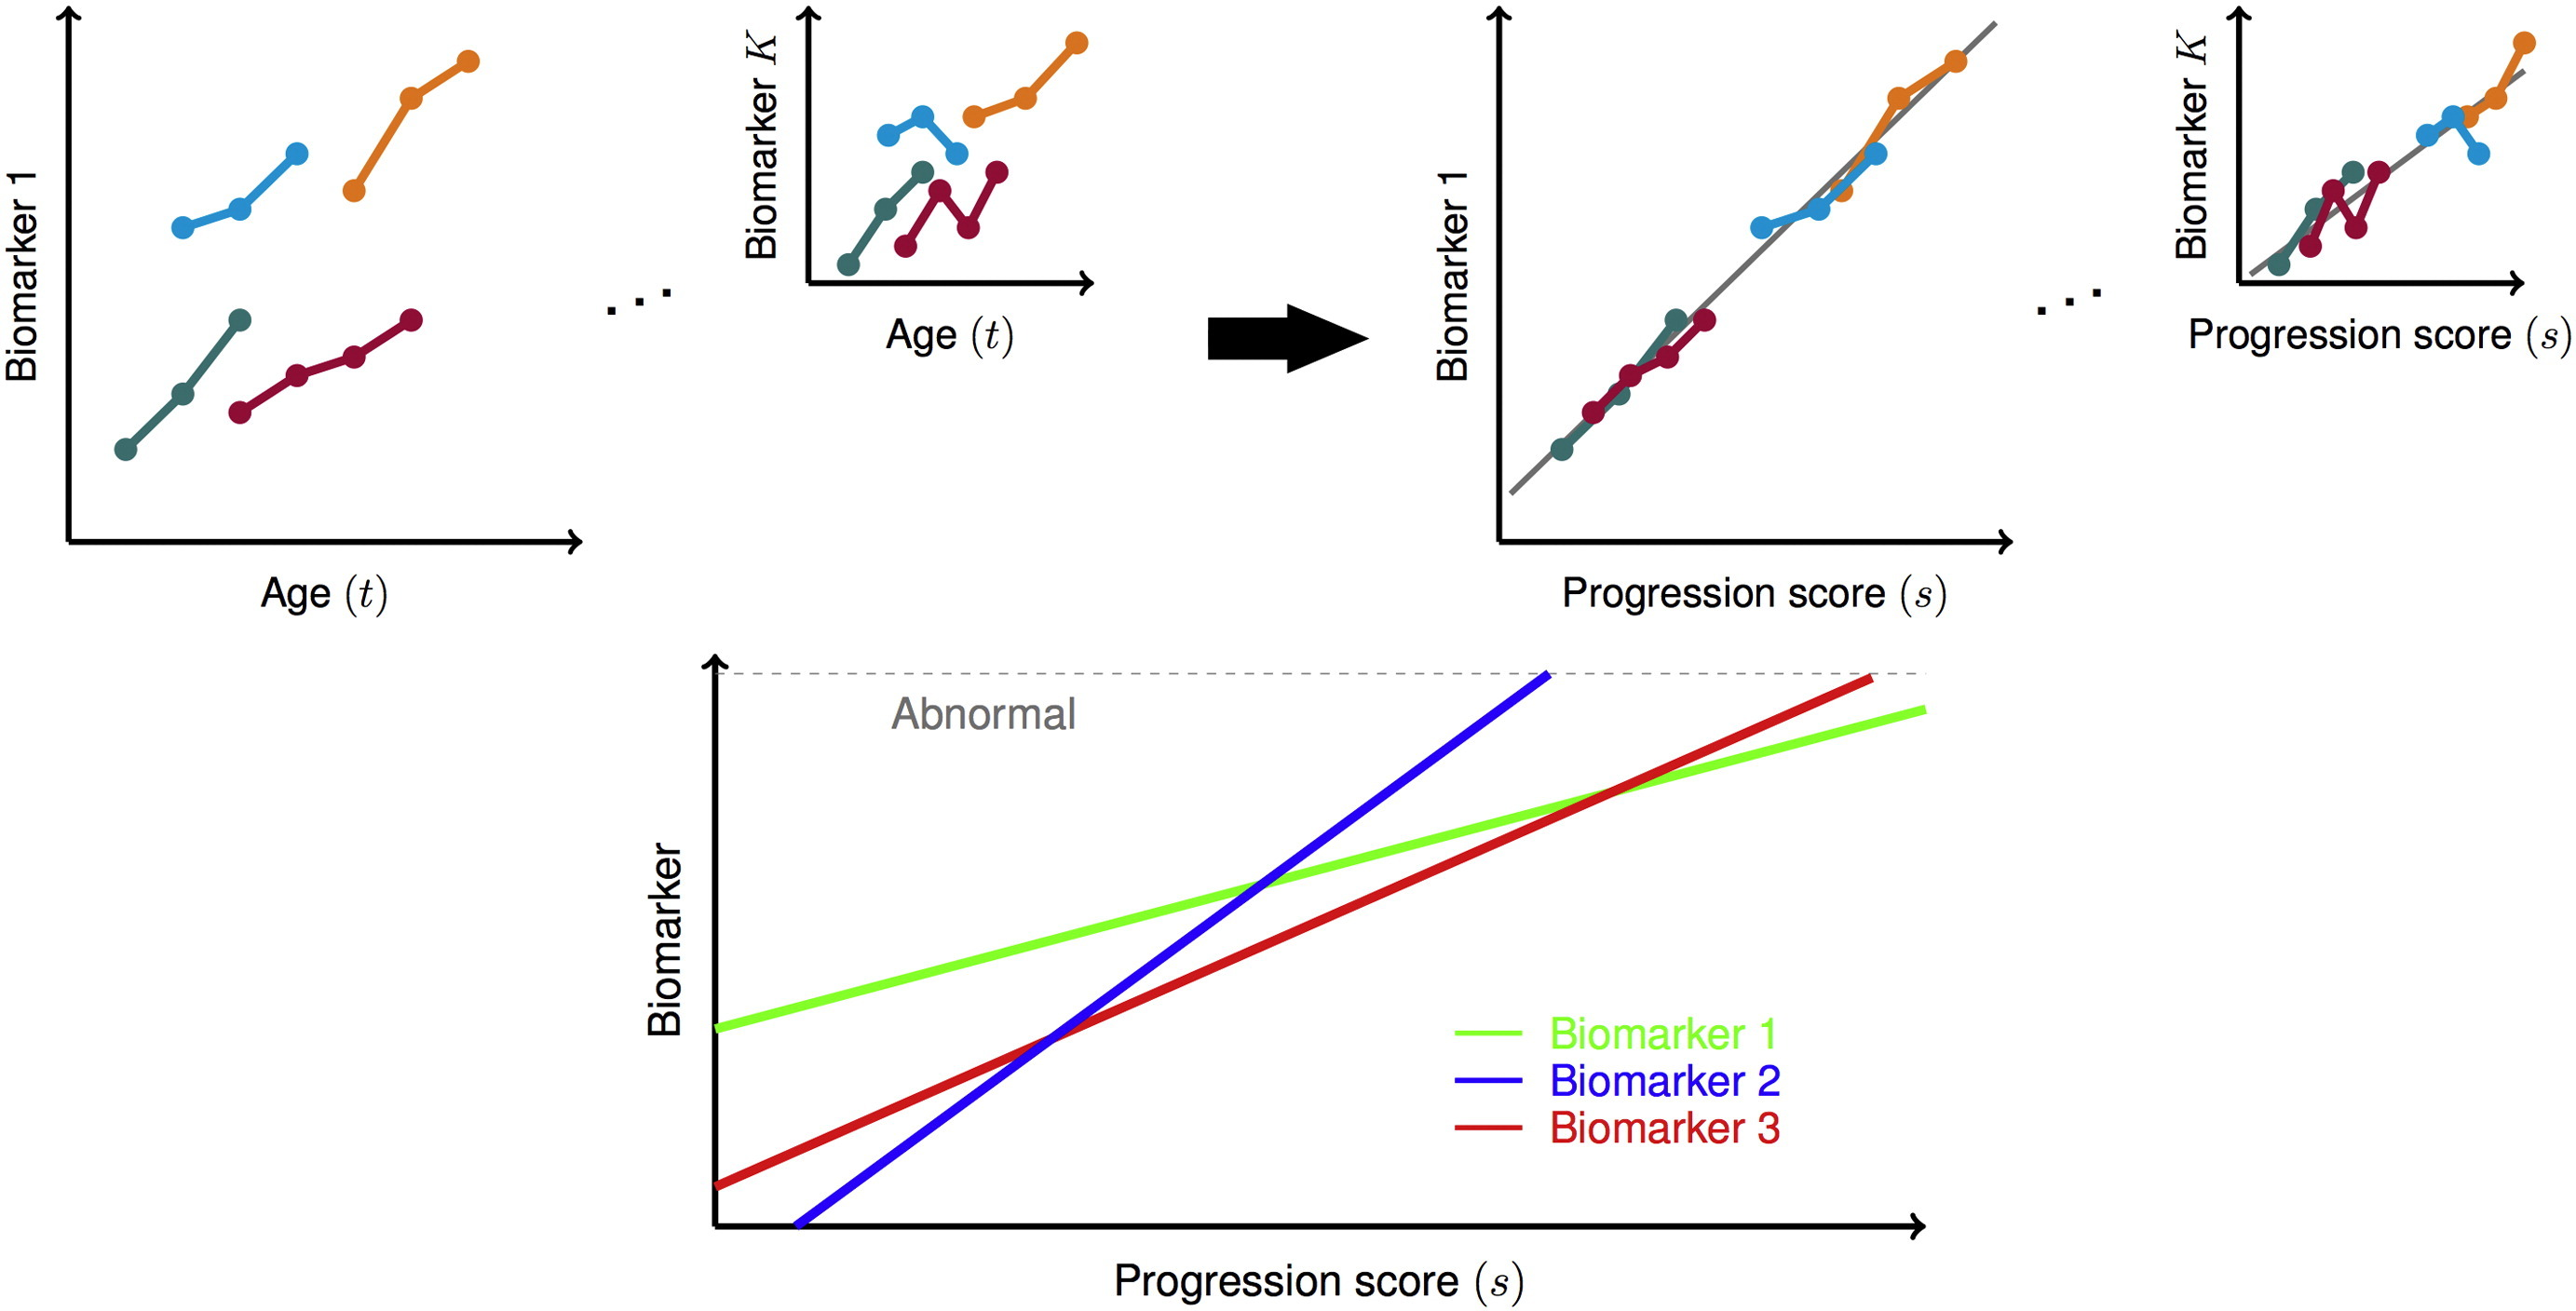
\includegraphics[width=0.8\textwidth]{images/bilgelDiagram}
\caption[Voxelwise disease progression model by Bilgel et al. \cite{bilgel2016multivariate}]{Diagram of the voxelwise disease progression model by Bilgel et al. \cite{bilgel2016multivariate}. The model places biomarker measurements along a latent "progression score" axis, and then models the dynamics of these measurements using linear functions. Reproduced with permission from \cite{bilgel2016multivariate}.}
\label{fig:bckBil}
\end{figure}

A voxelwise disease progression model has been introduced in 2016 by Bilgel et al. \cite{bilgel2016multivariate}. This model allows the discovery of patterns of atrophy that are not confined to a given region of interest (ROI). Since the input data is represented by voxel-wise measurements such as amyloid burden, a spatial correlation function is used to model correlation between voxel values. The model is built on the framework of the disease progression score by Jedynak et al. \cite{jedynak2012computational}. 

A diagram of the model is given in Fig \ref{fig:bckBil}. The model aligns biomarker measurements along a latent "progression score" axis, and then models the dynamics of these measurements using linear functions. Let us assume that $t_{ij}$ represents the age for subject $i$ at visit $j$. The progression score $s_{ij}$ for subject $i$ at visit $j$ is an affine transformation of age $t_{ij}$:

\begin{equation}
 \begin{cases}
 s_{ij} = \alpha_i t_{ij} + \beta_i = \textbf{q}_{ij}^T\textbf{u}_i\\
 \textbf{u}_i \sim N_2(\textbf{m}, V(\boldsymbol{\nu}))
\end{cases}
\end{equation}
where $\alpha_i$, $\beta_i$ are the progression speed and time shift of subject $i$, $\textbf{q}_{ij} = [t_{ij}, 1]^T$ and $\textbf{u}_{i} = [\alpha_i, \beta_i]^T$. The prior covariance matrix $V$ is modelled as a 2 $\times$ 2 positive definite matrix that has a Log-Cholesky parametrisation given by $\boldsymbol{\nu}$. More precisely, if we consider a matrix $U$ such that $V = UU^T$ and $U = \begin{bmatrix}
    U_{11} & U_{12} \\
    0 & U_{22}\\
\end{bmatrix}$, then $\boldsymbol{\nu} = [logU_{11}, logU_{12}, logU_{22}]$

Furthermore, let us denote by $\textbf{y}_{ij}$ the $K \times 1$ vector of biomarker measurements for subject $i$ at visit $j$. The longitudinal trajectories corresponding to these measurements are modelled as follows:

\begin{equation}
 \begin{cases}
  \textbf{y}_{ij} = \textbf{a}s_{ij}+\textbf{b}+\epsilon_{ij}\\
  \epsilon_{ij} \sim N_K(0,R(\boldsymbol{\lambda},\boldsymbol{\rho}))
 \end{cases}
\end{equation}
where $\textbf{a} = [a_1, \dots, a_K]^T$, $\textbf{b} = [b_1, \dots, b_K]^T$ are the coefficients of the linear model and $\epsilon_{ij}$ is the measurement noise that is independent and identically distributed across different subjects and visits. The matrix $R(\boldsymbol{\lambda},\boldsymbol{\rho})$ is the spatial covariance that is assumed to have the form $R = \Lambda C \Lambda$, where $\Lambda$ is a diagonal matrix with diagonal elements $\boldsymbol{\lambda}$ and $C$ is a correlation matrix that is parameterised by $\boldsymbol{\rho}$ \cite{bilgel2016multivariate}. This ensures that the matrix $R(\boldsymbol{\lambda},\boldsymbol{\rho})$ is positive definite. In order to model correlation among voxel measurements, the elements $C_{kk'}$ of matrix $C$ must be a function of the distance $d \equiv d(k,k')$ between voxels $k$ and $k'$. Several such options exist:
\begin{itemize}
 \item Exponential: $C_{kk'} = \text{exp}(-d/\rho)$
 \item Gaussian: $C_{kk'} = \text{exp}(-(d/\rho)^2)$
 \item Exponential: $C_{kk'} = \left(1+(d/\rho)^2\right)^{-1}$
 \item Spherical: $C_{kk'} = \left( 1 - \frac{3}{2}\frac{d}{\rho} + \frac{1}{2}\left(\frac{d}{\rho}\right)^{3} \right)$ if $d<\rho$
\end{itemize}
The model parameters are therefore $\boldsymbol{\theta} = [\textbf{m},\boldsymbol{\nu},\textbf{a},\textbf{b},\boldsymbol{\lambda},\boldsymbol{\rho}]$. The model is a mixed effects model where $\textbf{a}$, $\textbf{b}$ are the fixed effects and $\textbf{u}_i$ are the random effects. 

\subsubsection{Model Fitting}

The model is fit using the Expectation-Maximisation (EM), described below. In line with the standard EM framework \cite{bishop2007pattern}, the algorithm optimises the expected value of the full log-likelihood $\mathbb{E}_{p(\textbf{u}|\theta')}\left[l(\textbf{y}, \textbf{u}; \boldsymbol{\theta})\right]$ given the current estimate of the latent variables $\textbf{u}$. The complete data log-likelihood is:
\begin{align*}
 & l(\textbf{y}, \textbf{u}; \boldsymbol{\theta}) = \sum_i l(\textbf{y}_i, \textbf{u}_i; \boldsymbol{\theta}) =\\
 & -\frac{1}{2}\sum_{i,j}log|2\pi R|-\frac{1}{2}\sum_{i,j}\left(\textbf{y}_{ij}-Z_{ij}\textbf{u}_i-\textbf{b}\right)^T \\
 & -\frac{1}{2}\sum_{i} log|2\pi V|-\frac{1}{2}\sum_{i}(\textbf{u}_i-\textbf{m})^T V^{-1}(\textbf{u}_i-\textbf{m})
 \numberthis \label{eq:bilgel3}
\end{align*}

\textbf{E-step}

Let $(\textbf{y}, \textbf{u})$ be the complete data and $\boldsymbol{\theta}' = [\textbf{m}',\boldsymbol{\nu}',\textbf{a}',\textbf{b}',\boldsymbol{\lambda}',\boldsymbol{\rho}']$ be the parameters estimated at the previous EM iteration. Bilgel et al. \cite{bilgel2016multivariate} show that the E-step integral $Q(\boldsymbol{\theta}, \boldsymbol{\theta}')$ is proportional to $\sum_i \int \Phi(\tilde{\textbf{u}_i};\hat{\textbf{u}}'_i, \Sigma_i') l(\textbf{y}_i, \tilde{\textbf{u}}_i; \boldsymbol{\theta})d\tilde{\textbf{u}}_i$, where $\Phi$ is a multivariate normal probability density function with mean:

\begin{equation}
 \hat{\textbf{u}}'_i = \left( \sum_{j} Z'^T_{ij} R'^{-1} Z'_{ij} + V'^{-1}\right)^{-1}\left( \sum_{j} Z'^T_{ij} R'^{-1} (\textbf{y}_{ij}-\textbf{b}') + V'^{-1}\textbf{m}' \right)
\end{equation}
and covariance matrix $\Sigma'_{i}=\left( \sum_{j} Z'^T_{ij} R'^{-1} Z'_{ij} + V'^{-1}\right)^{-1}$. Evaluating the integral gives the following final form:

\begin{align*}
 & Q(\boldsymbol{\theta}, \boldsymbol{\theta}') = -\frac{1}{2} \sum_{ij}log|R| - \frac{1}{2}\sum_{ij}\left( \textbf{y}_{ij} - Z_{ij}\hat{\textbf{u}}'_i -\textbf{b}\right) - \frac{1}{2}\sum_{ij}Tr\left( Z^T_{ij} R^{-1} Z_{ij}\Sigma_i' \right) - \\
 & \frac{1}{2}\sum_{i}log|V| - \frac{1}{2}\sum_{i}\left( \hat{\textbf{u}}'_i - \textbf{m} \right)^T V^{-1} \left( \hat{\textbf{u}}'_i - \textbf{m} \right) - \frac{1}{2}\sum_i Tr\left( V^{-1} \Sigma_i'\right) \numberthis \label{eq:bilgel_e-step}
\end{align*}


\textbf{M-step}

At the M-step we need to find $\boldsymbol{\theta} = \argmax_{\boldsymbol{\theta}}Q(\boldsymbol{\theta}, \boldsymbol{\theta}')$. The full derivations are given in \cite{bilgel2016multivariate}, yielding the following updates:

\begin{equation}
\label{eq:bilgel_mstep1}
 \textbf{a} = \frac{\left( \sum_i \nu_i \right) \left( \sum_{ij} \textbf{y}_{ij}s'_{ij} \right) - \left( \sum_{ij} \textbf{y}_{ij} \right) \left( \sum_{ij}s'_{ij} \right)}{\left( \sum_i \nu_i \right) \left( \sum_{ij} \textbf{q}_{ij}^T \Sigma_i' \textbf{q}_{ij} + s_{ij}'^2 \right) - \left( \sum_{ij}s'_{ij} \right)^2}
\end{equation}

\begin{equation}
\label{eq:bilgel_mstep2}
 \textbf{b} = \frac{\left( \sum_{ij} \textbf{y}_{ij} \right) \left( \sum_{ij} \textbf{q}_{ij}^T \Sigma_i' \textbf{q}_{ij} + s_{ij}'^2 \right) - \left( \sum_{ij} \textbf{y}_{ij}s'_{ij} \right) \left( \sum_{ij} s'_{ij} \right)}{\left( \sum_i \nu_i \right) \left( \sum_{ij} \textbf{q}_{ij}^T \Sigma_i' \textbf{q}_{ij} + s_{ij}'^2 \right) - \left( \sum_{ij}s'_{ij} \right)^2}
\end{equation}

\begin{equation}
 \textbf{m} = \frac{1}{n}\sum_i \hat{\textbf{u}}'_i
\end{equation}

\begin{equation}
 \boldsymbol{\nu} = \argmax_{\boldsymbol{\nu}} Q(\boldsymbol{\theta}, \boldsymbol{\theta}')
\end{equation}

\begin{equation}
 \boldsymbol{\lambda}, \boldsymbol{\rho} = \argmax_{\boldsymbol{\lambda}, \boldsymbol{\rho}} Q(\boldsymbol{\theta}, \boldsymbol{\theta}')
\end{equation}

\subsubsection{Advantages and Limitations}

The model by Bilgel et al. \cite{bilgel2016multivariate} has several advantages. First of all, it is specifically tailored for dealing with voxelwise measurements such as amyloid load by modelling the spatial correlations. Secondly, like the disease progression score by Jedynak et al. \cite{jedynak2012computational}, it estimates subject specific temporal shifts and progression speeds. 

The model has several limitations. First of all, the biomarker trajectories are assumed to be linear, which is a strong assumption especially for early biomarkers such as amyloid, which start to plateau when subjects are in the MCI stages. The linearity was required in order to make the model inference with EM computationally tractable. Moreover, the biomarker correlation structure based on a spatial distance function does not allow one to recover fine-grained, disconnected patterns of pathology, as has been found for various types of dementias due to disruption in underlying brain networks \cite{seeley2009neurodegenerative}. The model also doesn't account for inter-subject differences by estimating deviations from the common population-wide trajectory.

\subsection{Cortical Atrophy Progression Model}
\label{sec:bckCor}

\begin{figure}
\centering
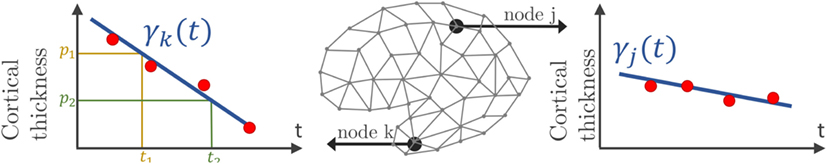
\includegraphics[width=0.8\textwidth]{images/kovalDiag1}

\vspace{2em}
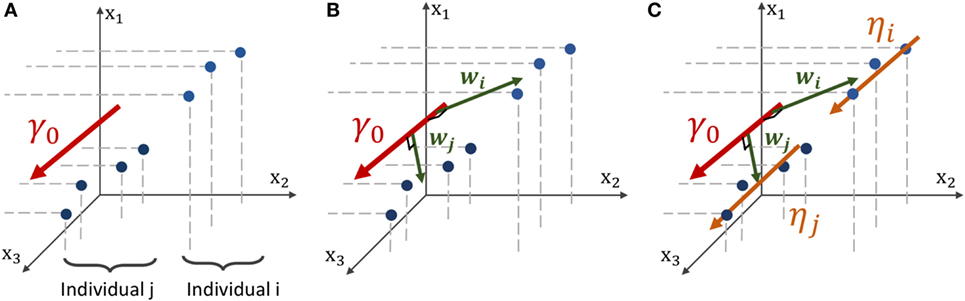
\includegraphics[width=0.8\textwidth]{images/kovalDiag2}
\caption[Diagram of the cortical atrophy progression model by Koval et al. \cite{koval2017statistical}]{Diagram of the cortical atrophy progression model by Koval et al. \cite{koval2017statistical}. (top) The model estimates a unique, linear trajectory for the dynamics of cortical thickness measurements at each point on the brain cortical surface. (bottom) Subject-specific trajectories $\eta_i$ and $\eta_j$ are modelled by a shift of the population trajectory $\gamma_0$ through vectors $w_i$ and $w_j$. Reproduced with permission from \cite{koval2017statistical}.}
\label{fig:bckKov}
\end{figure}

The cortical atrophy progression model was introduced by Koval et al.  \cite{koval2018spatiotemporal}. A diagram of the model is given in Fig. \ref{fig:bckKov}. The model estimates vertexwise linear trajectories of cortical thickness over the entire population, accounting for latent subject specific time-shifts. The equation modelling a biomarker measurement $y_{ijk}$ for subject $i$ at visit $j$ for location $k$ on the brain surface is given as:

\begin{equation}
y_{ijk} = p_k + w_{ik} + \nu_k\alpha_i(t_{ij} - \tau_i - t_0) + \epsilon_{ijk}
\end{equation} 
where $p_k$ and $\nu_k$ are parameters of the linear trajectory over the latent space specific to location $k$, $w_{ik}$ is a subject and location specific intercept, $\tau_i$ is the time-shift for subject $i$, $t_0$ is a time-shift reference and $\epsilon_{ijk}$ is the Gaussian noise for the $y_{ijk}$ measurement. In order to account for spatial correlation, a set of control nodes $\mathbb{V_c}$ is defined, which is a subset of all nodes $V$. Only for these control nodes will parameters $p_k$ and $\nu_k$ be estimated. For the other nodes, the parameters will be an interpolation of the parameters of the control nodes, weighted by the distance of that node to the control nodes. 

\subsection{Parameter Estimation}

Parameter estimation is done using the Monte-Carlos Markov-Chain Stochastic Approximation Expectation Maximisation (MCMC-SAEM) algorithm. This method essentially approximates the intractable E-step using the MCMC sampler. The optimisation method is proven to converge if the model belongs to the exponential family \cite{koval2017statistical}.

\subsection{Advantages and Limitations}

The model by Koval et al. has several advantages. It can estimate spatiotemporal patterns of atrophy, and can be extended to other types of voxelwise biomarkers such as amyloid load or DTI measures. The model also estimates subject-specific latent time-shifts, accounting for different but unknown ages of disease onset in distinct subjects. 

The model also has some limitations that need to be addressed in future work. One limitation is that the authors need to define a-priori the number of control points, which can affect the final smoothness level of the estimated patterns of pathology. While the authors only applied it to a brain surface made of 2,000 nodes, it is unclear whether the model can scale to higher resolutions.

\section{Mechanistic Models}
\label{sec:bckMec}

\subsection{The Network Diffusion Model}
\label{sec:bckNet}

\begin{figure}[h]
\centering
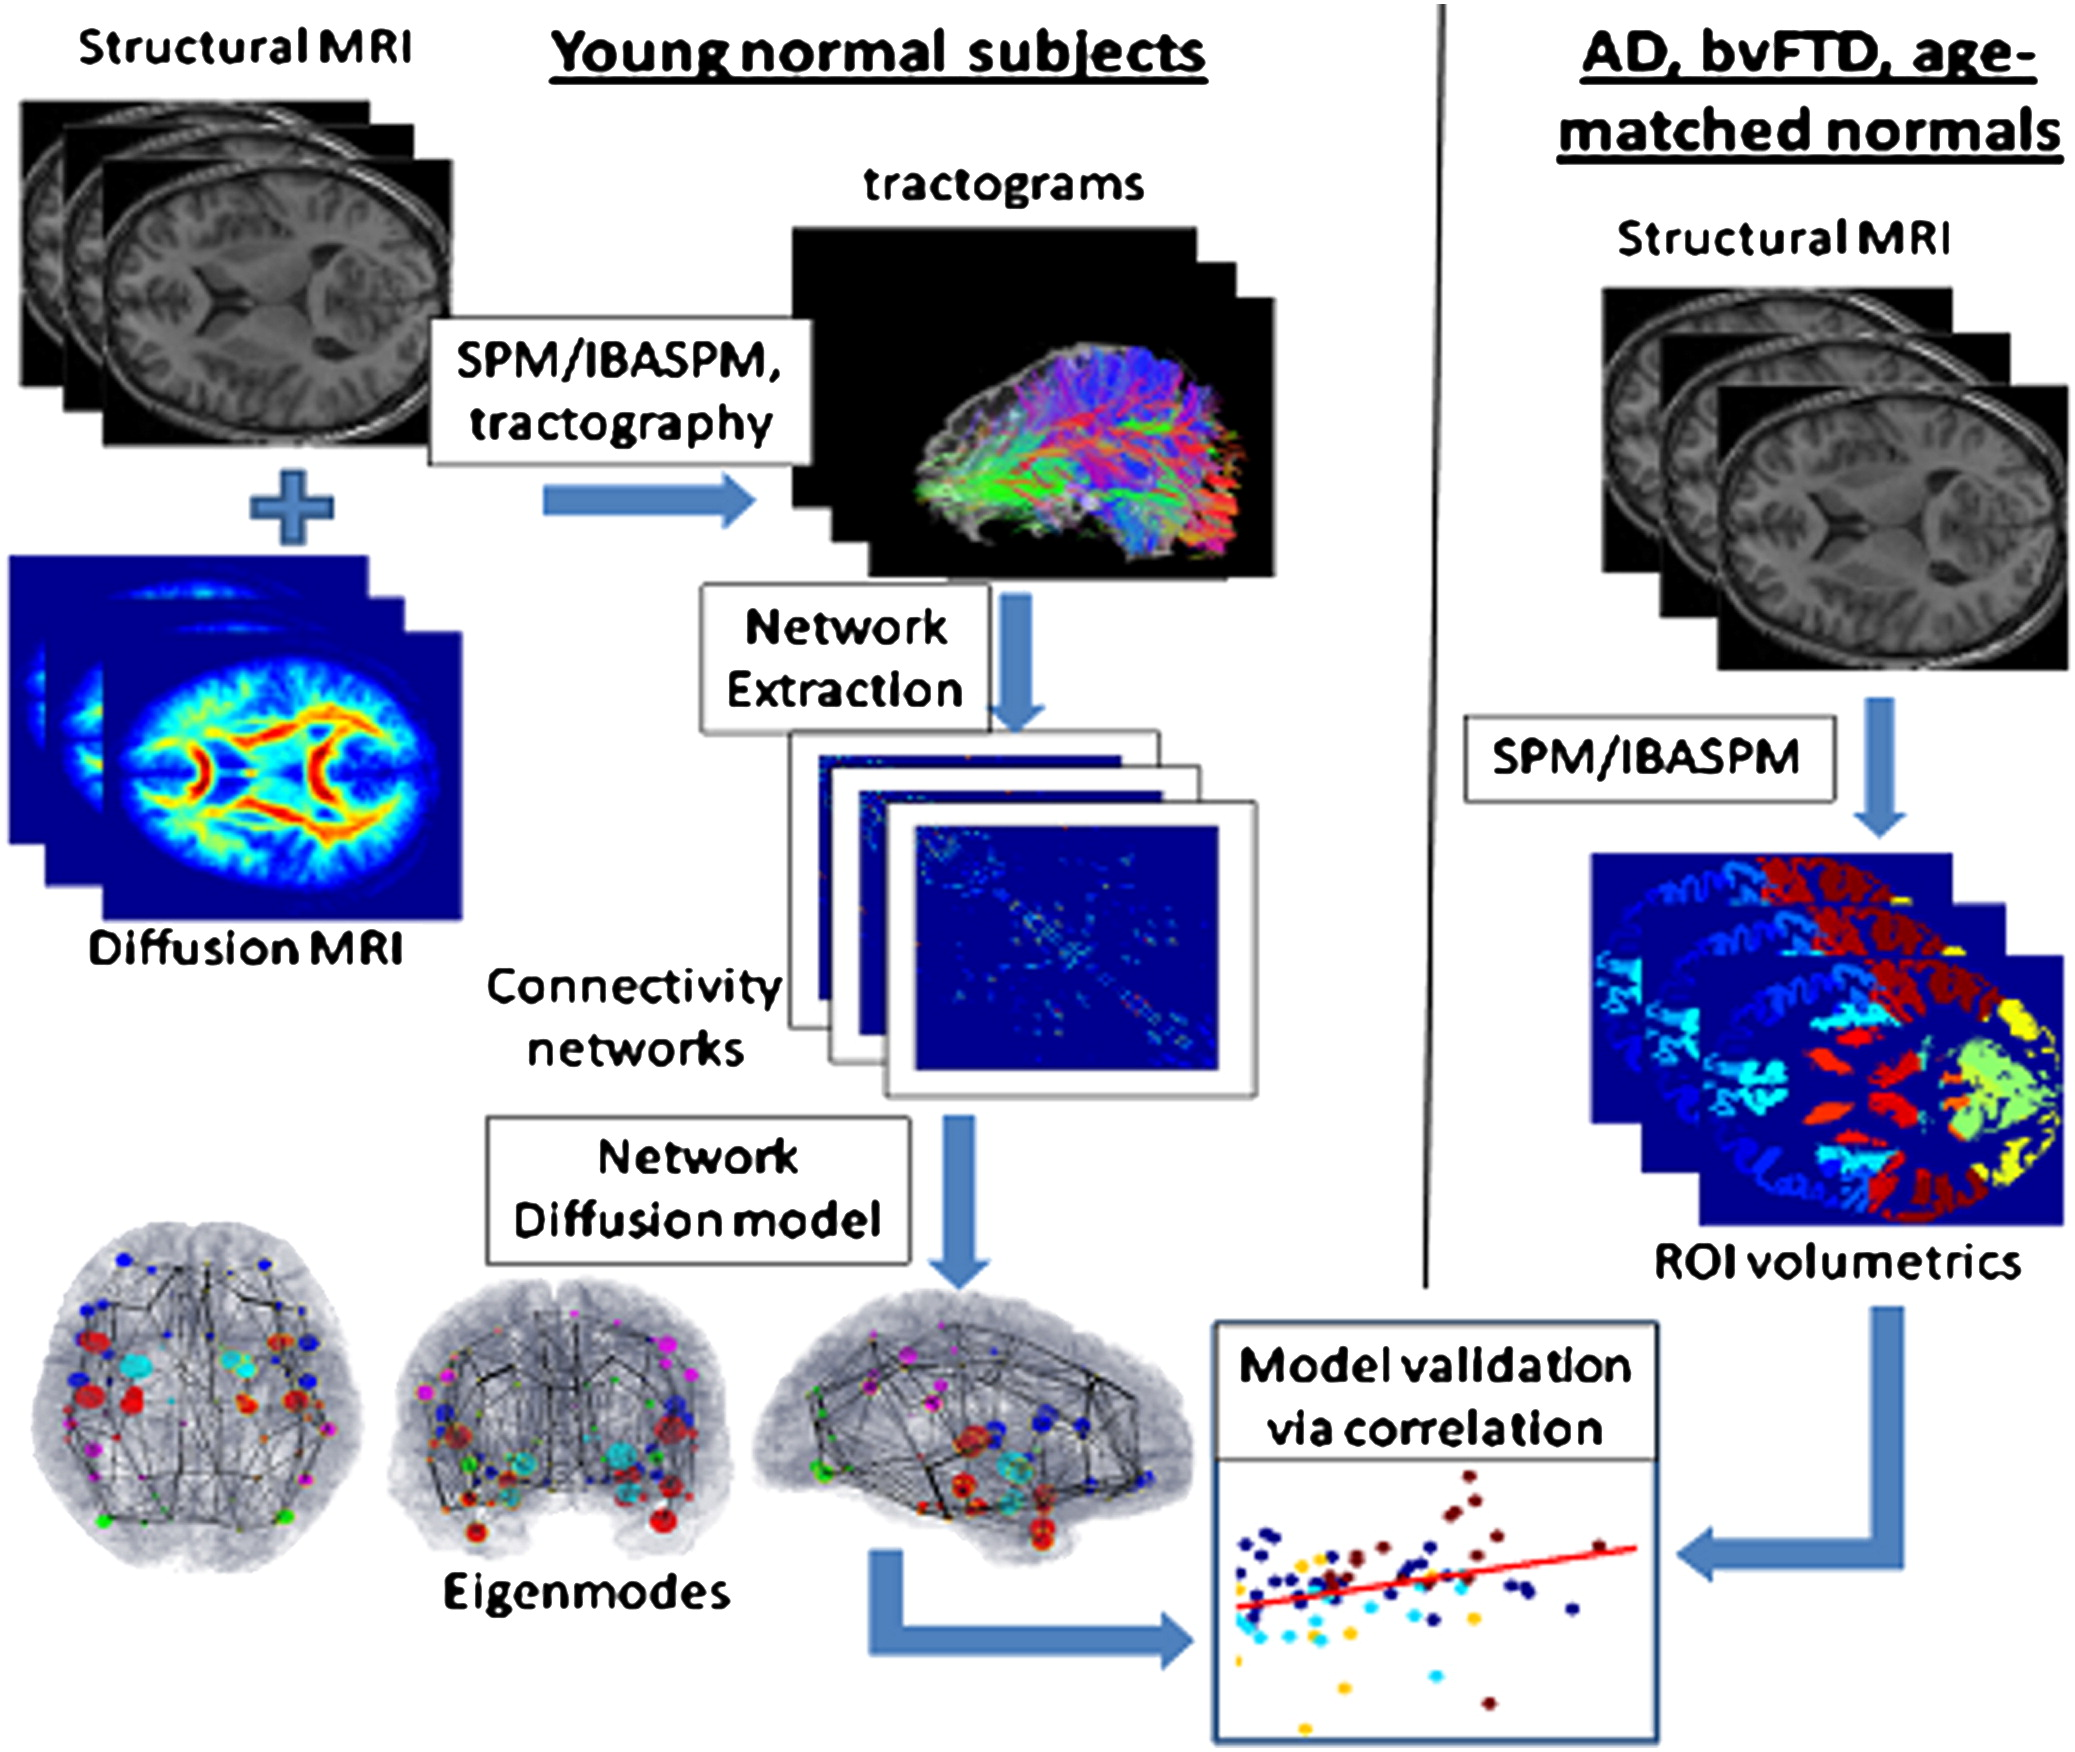
\includegraphics[width=0.8\textwidth]{images/rajDiag}
\caption[Diagram of the network diffusion model by Raj et al. \cite{raj2012network}.]{Diagram of the network diffusion model by Raj et al. \cite{raj2012network}. The model uses MRI and DTI data to extract a structural connectome from healthy subjects through tractography, then computes a connectivity network. Each network is represented as a graph where nodes represent brain ROIs where there is a certain concentration of toxic pathogens and edges represent the connectivity strength. Using this matrix, the authors estimate the eigenvectors of the graph, also called eigenmodes, which are then shown to correlate with atrophy patterns in normal ageing, AD and bvFTD. More precisely, for each disease they compute the amount of atrophy within each ROI corresponding to the graph nodes, and then correlate with the eigenmodes. Reproduced with permission from \cite{raj2012network}.}
\label{fig:bckRaj}
\end{figure}

The network diffusion model was introduced by Raj et al. in 2012 \cite{raj2012network} and later extended in 2015 \cite{raj2015network}. The model is inspired by evidence that Alzheimer's disease pathology spreads along vulnerable pathways in a prion-like manner rather than by spatial proximity \cite{villain2010sequential, englund1988white, kuczynski2010white}. The model works by simulating the diffusion process of a pathogenic protein along a structural connectivity graph from healthy controls. Atrophy and other higher-level pathogenic processes are assumed to be a product of the lower-level diffusion process. See Fig \ref{fig:bckRaj} for a diagram of the model.

The diffusion process is modelled on a hypothetical brain network $G = \{V, E\}$ whose nodes $v_i \in V$ represent regions-of-interest and edges $(i,j)$ having weight $c_{ij}$ represent fibre connections between regions $i$ and $j$. Structures $v_i$ are parcellated regions-of-interest obtained from an atlas, while the connection strength $c_{ij}$ is measured using tractography \cite{behrens2007probabilistic}. If we denote the disease factor in region $i$ as $x_i$, then the flow of the disease from a region $i$ to another region $j$ in a short time interval $\delta t$ is $\beta(x_i - x_j)c_{ij}\delta t$, where $\beta$ is a diffusivity constant controlling the diffusion speed. As $\delta t \to 0$, this results in the following first-order differential equation:
\begin{equation}
\label{eq:raj1}
 \frac{dx_j}{dt} = \beta c_{ij}(x_i - x_j)
\end{equation}
Now let us denote by $\textbf{x}(t) = \{x(v,t), v \in V \}$ the disease factor at time $t$ in every node of the network. Eq. \ref{eq:raj1} will then translate into the "network heat equation" \cite{kondor2002diffusion}:

\begin{equation}
\label{eq:raj2}
 \frac{d\textbf{x}(t)}{dt} = \beta H \textbf{x}(t)
\end{equation}
where $H$ is the Laplacian matrix of $G$ defined as:

\begin{equation}
\label{eq:raj3}
 H(i,j) = \begin{cases} 
 \sum_{j' \neq i} c_{ij'} & \mbox{for } i = j \\ 
 -c_{ij} & \mbox{otherwise} \\ 
\end{cases} 
\end{equation}
We model the cortical atrophy in region $k$ as the accumulation of the disease process:
\begin{equation}
\label{eq:raj4}
 \phi_k(t) = \int_0^t x_k(\tau)d\tau
\end{equation}
Extending this to the whole brain gives:
\begin{equation}
 \boldsymbol{\Phi(t)} = \int_0^t \textbf{x}(\tau)d\tau
\end{equation}
The solution to the above equation is given by:
\begin{equation}
 \textbf{x}(t) = \text{exp}(-\beta H t) \textbf{x}_0
\end{equation}
where $\textbf{x}_0$ is the initial disease concentration, where the term $\text{exp}(-\beta H t)$ acts as a smoothing operator. Performing eigenvalue decomposition on $H = U\Lambda U^{\dagger}$, where $U = [\textbf{u}_1,\dots,\textbf{u}_N]$ is the matrix of eigenmodes, allows to express $\textbf{x}(t)$ as:
\begin{equation}
 \textbf{x}(t) = U \text{exp}(-\Lambda \beta t) U^{\dagger} \textbf{x}_0 = \sum_{i=1}^N \left( \text{exp}(-\beta \lambda_i t) \textbf{u}_i^{\dagger} \textbf{x}_0 \right) \textbf{u}_i
\end{equation}
The time evolution of atrophy can then be described as:
\begin{equation} 
 \boldsymbol{\Phi}(t) = \int_0^t \sum_{i=1}^N \left( \text{exp}(-\beta \lambda_i t) \textbf{u}_i^{\dagger} \textbf{x}_0 \right) \textbf{u}_i\ dt = \sum_{i=1}^N \frac{1}{\beta \lambda_i} \left( 1-\text{exp}(-\beta \lambda_i t)\right) \textbf{u}_i^{\dagger} \textbf{x}_0 \textbf{u}_i 
\end{equation}
Raj et al. \cite{raj2012network} present evidence to suggest that the eigenmodes $\textbf{u}_i$ with the highest corresponding eigenvalues $\lambda_i$ represent the areas that are normally affected by key neurodegenerative processes or diseases, such as normal ageing, AD and behavioural variant frontotemporal dementia (bvFTD) respectively. They suggest that these areas are selectively vulnerable to these types of dementia, in line with previous theories in the field \cite{seeley2009neurodegenerative, zhou2010divergent, zhou2012predicting}. 

\subsubsection{Advantages and Limitations}

The diffusion model by Raj et al. \cite{raj2012network} has several advantages. In contrast with the models presented above, it is able to model the propagation of atrophy along brain connectomes, which can be used to test prion hypothesis or other related mechanisms. Secondly, this approach allows one to test for other hypotheses of network-based pathology spread such as nodal stress, transneuronal spread, trophic failure, and shared vulnerability \cite{zhou2012predicting}.

The model has several limitations. The model assumes static networks, even though the network dynamically evolves during the time course of the disease. The model also assumes a parametric form of the biomarker trajectories, either exponential or sigmoidal. 

\section{Machine Learning Methods}
\label{sec:bckMac}

Popular machine learning methods that are normally used for discriminative tasks can also be extended to model disease progression by estimating continuous variables. One such method is the Support Vector Machine, which is a non-probabilistic binary linear classifier that was originally developed by Vladimir N. Vapnik and Alexey Ya. Chervonenkis \cite{vapnik2006estimation}. They can perform non-linear classification by mapping the input data into higher-dimensional feature spaces using the \emph{kernel trick} and finding the hyperplane that optimally separates the data. They have been successfully used for differential diagnosis of different types of dementia using post-mortem confirmed subjects \cite{kloppel2008automatic}. Other uses of SVMs on medical images and other high-dimensional data have also been shown \cite{lao2004morphological,fan2005classification,mourao2005classifying,kawasaki2007multivariate}.

Other popular classifiers used in the machine learning field are random forests \cite{ho1995random,breiman2001random}. These work by building a multitude of decision trees on training data, using them to make predictions on the test data and performing majority voting on the predictions of individual trees to select the final labels. Random forests have been demonstrated in medical imaging for diagnosis classification \cite{gray2013random}, image quality transfer \cite{alexander2014image} or myocardium segmentation \cite{lempitsky2009random}. 

Yet another machine learning model popular for time-series predictions is the Long short-term memory (LSTM) network \cite{hochreiter1997long}. LSTMs are a type of recurrent artificial neural network (RNN) that replace the conventional hidden nodes from RNNs with \emph{memory cells}, which ensure that the gradient cannot vanish or explode during training. LSTMs have been applied in medical imaging research for diagnosing between healthy and AD subjects \cite{karlekar2018detecting}, predicting the onset of diseases \cite{razavian2016multi}, predicting diagnoses in electronic health records (EHR) \cite{lipton2015learning}, predicting mortality risk \cite{aczon2017dynamic} as well as several other clinical variables \cite{harutyunyan2017multitask}. 

\subsection{Advantages and Limitations}

Discriminative models such as SVMs, random forests or LSTMs have several advantages. They work for a wide variety of problems, datasets and underlying models and are generally robust to high-dimensional data. Some of them can also be resistant to overfitting, especially when used in conjunction with regularisation and data augmentation techniques. A key advantage of LSTMs in particular is that they are suitable for time-series data, and can be naturally used to predict future biomarker values, although the other models can also be extended to work with continuous data.

These discriminative models also have several limitations. First of all, they generally require labelled data, in the form of a-priori defined clinical categories or stages, which are usually coarse, inaccurate and biased. These limit the temporal resolution of the model. Moreover, it is also harder to interpret what these models learn from the data, which limits their use for understanding the disease process. For some models there is also a lack of mathematical proofs and guarantees regarding their convergence during training, as well as behaviour while making predictions.

\section{Summary}

In Fig. \ref{tab:compDPMs} we show a summary of the main features of data-driven disease progression models, as well as discriminative models. For each model, we show the trajectory shape, indicate whether models incorporated latent subject-specific time-shifts (in terms of intercept or intercept + progression speed), subject-specific trajectories in the form of random effects as well as spatial correlation. For each model, we also indicate the key limitation.

We can observe several key differences between the models. In terms of time-shifts, some models such as the DEM or the network diffusion model do not incorporate any time-shifts, although these could be extended to incorporate such time-shifts. Other models do not model subject-specific trajectories through random effects. Moreover, only spatiotemporal or mechanistic models incorporate correlation between different biomarker measurements. 

In conclusion, over the last few years there have been several models of disease progression that were developed, starting from the early comparisons based on symptomatic groups and moving on to more data-driven approaches and spatiotemporal models. Further work will focus on developing more mechanistic models that enable understanding of the underlying disease process, and can help guide drug development. One example of this is the recent work of \cite{georgiadis2018computational}, which models the dynamics of pathogenic proteins in a neural network and can help understand the effects of such pathogenic proteins in neurodegeneration. However, validation of such models is required through \emph{in vitro} and \emph{in vivo} studies. 

In the following chapters, I will present the application of some of these models to estimate the progression of Posterior Cortical Atrophy (chapter \ref{chapter:pca}), as well as the development of two novel models of disease progression (chapters \ref{chapter:dive} and \ref{chapter:dkt}).

%\begin{landscape}


\definecolor{orange0}{rgb}{1, 0, 0}
\definecolor{orange1}{rgb}{0.66, 0.33, 0}
\definecolor{orange2}{rgb}{0.33, 0.66, 0}
\definecolor{orange3}{rgb}{0, 0.7, 0}

\definecolor{green1}{rgb}{0, 0.6, 0}
\definecolor{red1}{rgb}{0.6, 0, 0}
\newcommand{\xmark}{\ding{55}}%

\newcommand{\myyes}{\textcolor{green1}{\Large{\checkmark}}}
\newcommand{\myno}{\textcolor{red1}{\Large{\xmark}}}
% \newcommand{}{×}

\begin{table}
\centering
\footnotesize
\renewcommand{\arraystretch}{1.5}% Spread rows out...
\begin{tabular}{>{\centering\arraybackslash}p{2.8 cm} | >{\centering\arraybackslash}p{2.3 cm} | >{\centering\arraybackslash}p{1.5 cm} | >{\centering\arraybackslash}p{1.5 cm} | >{\centering\arraybackslash}p{2.0 cm} | >{\centering\arraybackslash}p{2 cm} | >{\centering\arraybackslash}p{2.5 cm}}
 Model & Trajectory shape & \multicolumn{2}{c|}{Subject Time-shifts} & \multirow{2}{2cm}{\centering Subject-specific trajectory} & \multirow{2}{2cm}{\centering Models Biomarker Correlation} & Main Limitation \\
 & & intercept & speed & & \\
 \Xhline{2\arrayrulewidth}
 Event-based Model & step-function & \myyes** & \myno & \myno & \myno & discrete time\\
  \hline
 Differential Equation Model & non-parametric & \myno * & \myno * & \myno & \myno  & univariate\\
  \hline
 Disease Progression Score & sigmoid & \myyes & \myyes & \myno & \myno & sigmoidal trajectory assumption \\
  \hline
 Self-Modelling Regression & non-parametric & \myyes & \myyes & \myyes & \myno & can overfit + identifiability\\
  \hline
 Manifold Model & linear, sigmoid & \myyes & \myyes & \myyes & \myno & user-defined trajectory assumption \\
  \hline
 Voxelwise Model & linear & \myyes & \myyes & \myno & \myyes & linear trajectory assumption\\
  \hline
 Cortical Atrophy Progression Model & linear & \myyes & \myyes & \myyes & \myyes & user-defined trajectory assumption\\
  \hline
 Network diffusion Model & exponential, sigmoidal & \myno * & \myno *&  \myno & \myyes & assumes static connectome + no time-shift\\


\end{tabular}
\caption[Comparison of features of various disease progression models.]{Comparison of features of various disease progression models. By subject-specific trajectories, we exclude deviations from the population-wide trajectory only due to time-shifts. While the models have many limitations, the ones mentioned here are the main ones according to our own opinion. (*) Models cannot be used for subject staging in their basic formulation, but extensions to the model can enable them to estimate subject-specific disease onset and progression speed. Comparison analysis made by me. (**) The subject-specific time-shift in the EBM is discreete and based on cross-sectional data only.}
\label{tab:compDPMs}
\end{table}
%\end{landscape}

